%! suppress = TooLargeSection
% A-posteriori benchmark report: representation study (H1/H2) for Doya-style
% continuous-time value-gradient control of delayed, non-Markovian dynamics.
% Compiles standalone: pdflatex h1h2_representation_benchmark.tex (twice).
% No project notation package; macros are defined locally below.
\documentclass[11pt]{article}
\usepackage[utf8]{inputenc}
\usepackage[T1]{fontenc}
\usepackage{amsmath, amssymb, amsfonts}
\usepackage{amsthm}
\usepackage{mathtools}
\usepackage{mathrsfs}
\usepackage[a4paper, margin=2.4cm]{geometry}
\usepackage{graphicx}
\usepackage{booktabs}
\usepackage{array}
\usepackage{multirow}
\usepackage{xcolor}
\usepackage{pgfplots}
\pgfplotsset{compat=1.17}
\usepackage[hidelinks]{hyperref}

% Permit line breaks after underscores in \texttt (the long file/run-directory names in the
% reproduction appendix). Affects only text-mode \_ , never math-mode subscripts.
\makeatletter
\renewcommand{\_}{\discretionary{\textunderscore}{}{\textunderscore}}
\makeatother
\emergencystretch=2em

% --- Single shared counter across all numbered environments (Bourbaki convention) ---
\theoremstyle{plain}
\newtheorem{theorem}{Theorem}[section]
\newtheorem{proposition}[theorem]{Proposition}
\newtheorem{corollary}[theorem]{Corollary}
\newtheorem{lemma}[theorem]{Lemma}
\theoremstyle{definition}
\newtheorem{definition}[theorem]{Definition}
\newtheorem{finding}[theorem]{Empirical finding}
\newtheorem{observation}[theorem]{Observation}
\newtheorem{remark}[theorem]{Remark}

\newcommand{\R}{\mathbb{R}}
\newcommand{\N}{\mathbb{N}}
\newcommand{\E}{\mathbb{E}}
\newcommand{\sig}{\mathbb{S}}
\newcommand{\rank}{\operatorname{rank}}
\newcommand{\effrank}{\operatorname{erank}}
\newcommand{\cond}{\operatorname{cond}}
\newcommand{\Cov}{\operatorname{Cov}}
\newcommand{\tr}{\operatorname{tr}}
\newcommand{\softplus}{\operatorname{softplus}}
\newcommand{\norm}[1]{\left\lVert #1 \right\rVert}
\newcommand{\abs}[1]{\left\lvert #1 \right\rvert}
\newcommand{\inner}[2]{\left\langle #1,\, #2 \right\rangle}
\newcommand{\half}{\tfrac12}
% verdict marks
\newcommand{\holds}{\textcolor{black!80}{\textbf{holds}}}
\newcommand{\failsv}{\textcolor{black!55}{fails}}

\title{Does history help, and does the path signature help?\\[3pt]
\large An a-posteriori benchmark of value-gradient representations for\\
continuous-time control of delayed, non-Markovian dynamics}
\author{Benchmark report --- \texttt{RL\_and\_signatures}}
\date{2026-06-30}

\begin{document}
\maketitle

\begin{abstract}
Three feature maps for the value function of a Doya-style continuous-time
value-gradient controller are benchmarked on a graded family of delayed (non-Markovian) plants,
by two complementary instruments: a comprehensive \emph{learned} study sweeping representation
capacity (polynomial degree, signature depth) across many examples and five seeds, and a
\emph{controlled} continuous-time optimal-control oracle protocol that isolates the
representational question by solving the fit exactly. (The originally-intended nonlinear-delayed
example, a continuous-stirred-tank reactor, is measured to be structurally near-Markovian and is
demoted; a delay-coupled Hopfield network replaces it.) Two hypotheses are tested by
the closed-loop cost $I$: $H_1$, that a representation of the \emph{history} window improves
on a representation of the current state alone; and $H_2$, that the \emph{path-signature}
structure improves on a plain polynomial of the history window. The first hypothesis
\holds\ wherever the delay genuinely couples the dynamics --- the linear delay equation, the
delayed Hopfield network, the five-vehicle platoon, and the Mackey--Glass oscillator --- and
\failsv\ exactly on the Markovian negative control, where all three representations coincide
at $I=3.115$ (measured, five seeds). The second hypothesis does \emph{not} hold. Early
single-seed evidence that the signature beats the history window on long-delay examples is shown
to be an artefact of \emph{under-sampling}: the degree-two history feature dimension grows as
$O(\tau^{2})$ with the delay $\tau$ (window $6\mapsto61$, dimension $90\mapsto7625$), so on a
long-delay example at fixed sample size the history fit is under-sampled. Under three controls ---
quadrupled data, Tikhonov conditioning, and off-sheet rebalancing --- the history
representation recovers and \emph{matches or beats} the signature on every example measured
(Hopfield at $\tau=3$: $I=0.289$ versus $0.323$; Mackey--Glass limit cycle at off/dim${}=4$:
$I=0.0108$ versus $0.0126$). The mechanism is the effective-rank phenomenon of the companion
note, proven as a Veronese bound and measured here: the controlled-trajectory feature Gram has
an effective rank that rises only from $3.3$ to $3.5$ across $\tau\in\{1,\dots,6\}$ while the
nominal dimension increases by a factor of $28$. The signature's sole genuine advantage is therefore
\emph{sample efficiency} --- a fixed feature dimension --- not representational power; and that
advantage reverses at high state-space dimension, where the signature's own $O(d^{L})$ channel
growth makes it the ill-conditioned representation (platoon: $I=0.227$ versus the history
window's $0.029$). Every number is read off a saved run; the reproduction appendix lists the
script and run directory behind each.
\end{abstract}

{\small\tableofcontents}

\section{Common framework}\label{sec:framework}

\emph{This section fixes, once, the objects shared by every test case: the control problem,
the oracle that plays the reference, the representations under test, the learning problem and
its data protocol, and the three metrics. The per-example sections that follow vary only the
plant.}

\subsection{The control problem and Doya's value-gradient law}

\begin{definition}[Controlled delay system and cost]\label{def:plant}
A plant is a controlled delay differential equation on $\R^{n}$,
\begin{equation}\label{eq:plant}
\dot x(t)=f\big(x(t),\,x(t-\tau),\,u(t)\big),\qquad x(s)=x_{0}(s)\ \ (s\in[-\tau,0]),
\end{equation}
with control $u(t)\in\R^{m}$ and a quadratic running cost
$\ell(x,u)=x^{\top}Qx+u^{\top}Ru$, $Q\succeq0$, $R\succ0$, regulating to the origin (a shifted
equilibrium). The closed-loop performance of a feedback law is the accumulated cost
\begin{equation}\label{eq:cost}
I=\int_{0}^{T}\ell\big(x(t),u(t)\big)\,\mathrm dt
\end{equation}
from a fixed deployment initial condition, integrated by the environment's own Runge--Kutta
solver. $I$ is the operative quantity: every verdict in this report is a comparison of $I$.
\end{definition}

\begin{definition}[Value-gradient feedback]\label{def:doya}
Let $J^{\ast}$ denote the optimal cost-to-go of \eqref{eq:plant}--\eqref{eq:cost} --- the minimal
accumulated cost \eqref{eq:cost} attainable from the current history --- and let the value be its
negative, $V^{\ast}:=-J^{\ast}$ (reward convention). Doya's continuous-time law sets the
control to the half-gradient of the value along the input channel,
\begin{equation}\label{eq:doyalaw}
u=\half\,R^{-1}B^{\top}\,\partial_{x}V^{\ast},\qquad B:=\partial_{u}f,
\end{equation}
which reproduces the optimal control exactly for the continuous-time value (no time-step
rescaling). A learned critic $V_{\theta}$ is deployed by the same law,
$u_{\theta}=\half R^{-1}B^{\top}\partial_{x}V_{\theta}$, so what is \emph{used} is the
\emph{gradient} $\partial_{x}V_{\theta}$, not $V_{\theta}$ itself --- a distinction that drives
the entire analysis (Section~\ref{sec:mechanism}).
\end{definition}

\subsection{The reference: the continuous-time oracle and its consistency check}

\begin{definition}[Continuous-time oracle]\label{def:oracle}
The reference controller is the continuous-time optimal control of \eqref{eq:plant}, built per
example.
\begin{itemize}
\item \emph{Linear / linearised examples (delayed-LQR).} The history segment $[-\tau,0]$ is
discretised at the $\nu+1$ Chebyshev collocation nodes $-\tau=\theta_{\nu}<\dots<\theta_{0}=0$, and
the augmented state $z=\big(x(t+\theta_{0}),\dots,x(t+\theta_{\nu})\big)\in\R^{n(\nu+1)}$ stacks the
state at those nodes. The delay equation \eqref{eq:plant} becomes the ordinary differential equation
$\dot z=Mz+\mathcal N u$, in which $M\in\R^{n(\nu+1)\times n(\nu+1)}$ collocates the transport
identity $\partial_{t}x=\partial_{\theta}x$ at the interior nodes and the linearised dynamics
$\dot x=A_{0}\,x(t)+A_{1}\,x(t-\tau)$ at the boundary node $\theta_{0}=0$, and
$\mathcal N=(B^{\top},0,\dots,0)^{\top}\in\R^{n(\nu+1)\times m}$ injects the control at that node. The
algebraic Riccati equation $M^{\top}P_{c}+P_{c}M-P_{c}\mathcal N R^{-1}\mathcal N^{\top}P_{c}+Q_{z}=0$,
with $Q_{z}$ equal to $Q$ on the boundary block and $0$ elsewhere, yields the value
$V^{\ast}(z)=-z^{\top}P_{c}z$ and the feedback $u^{\ast}=-K_{c}z$ with
$K_{c}=R^{-1}\mathcal N^{\top}P_{c}$. (\texttt{src/solvers/continuous\_oracle.py}.)
\item \emph{Nonlinear examples (Pontryagin).} On the same augmented state the two-point
boundary-value problem in $(z,\lambda)$ is solved, with $\lambda$ the costate; by the maximum
principle $\lambda(t)=\partial_{z}V^{\ast}$ is the value gradient, so
$u^{\ast}=-\half R^{-1}B^{\top}\lambda_{0}$ (with $\lambda_{0}$ the boundary block of $\lambda$) is
Doya's law \eqref{eq:doyalaw} evaluated on the exact value.
(\texttt{src/solvers/\{mackey\_glass,delayed\_hopfield\}\_pontryagin.py}.)
\end{itemize}
\end{definition}

\emph{Consistency check.} The oracle is accepted only after a numerical consistency check: on a
cloud of augmented states, Doya's law \eqref{eq:doyalaw} applied to the oracle value gradient must
reproduce the oracle feedback $u^{\ast}$ to machine precision --- direction cosine $1$ and
magnitude ratio $\norm{u}/\norm{u^{\ast}}=1$. Every example in this report passes this check to four
decimals (recorded as the \texttt{gate} field of each \texttt{summary.json}); an example whose oracle
failed it would be excluded.

The oracle is a deliberately strong, non-deployable adversary: it has the exact dynamics and
solves a boundary-value problem per window. It plays two roles --- it \emph{labels} the
training data with $(V^{\ast},u^{\ast})$, and it supplies the deployable linear-feedback
reference cost $I^{\ast}$ against which the learned $I$ is read.

\subsection{The two hypotheses}

With the three representations of Definition~\ref{def:reps} ranked markovian $\to$ raw-history
$\to$ signature, the two questions under test are the adjacent pairwise comparisons of the
closed-loop cost:
\begin{itemize}
\item $H_1$ (\emph{does history help?}): $I[\text{raw-history}]<I[\text{markovian}]$;
\item $H_2$ (\emph{does the signature structure help?}): $I[\text{signature}]<I[\text{raw-history}]$.
\end{itemize}
Each is recorded as holding on an example only if the contender lowers $I$ by more than a relative
margin of $3\%$; a near-tie is the negative result. The single-example verdict is indicative; the
falsifiable statement is the seed-resolved comparison of Section~\ref{sec:h1}.

\subsection{The representations under test}

\begin{definition}[Markovian, raw-history, signature critics]\label{def:reps}
The control-cadence history at time $t$ is the finite sequence
$\underline x=(x_{t-i\Delta t})_{0\le i\le L-1}\in(\R^{n})^{L}$ of the last $L$ state samples at the
control step $\Delta t$ --- $x_{t}$ the current state and $x_{t-(L-1)\Delta t}$ the oldest --- with
$L=\lceil\tau/\Delta t\rceil+1$ so the sequence spans the delay. The value critic is linear in a
feature map $\phi$, $V_{\theta}(\underline x)=\inner{\theta}{\phi(\underline x)}$, with the three maps
\begin{enumerate}
\item \emph{markovian} $\phi_{M}$: the degree-$2$ monomials of the \emph{current} state $x_{t}$
alone (no history);
\item \emph{raw-history} $\phi_{H}$: the degree-$2$ monomials of the \emph{whole} sequence
$\underline x$ (its $Ln$ scalar entries);
\item \emph{signature} $\phi_{S}$: the depth-$2$ path signature of the time-augmented sequence
$\big(i\Delta t,\,x_{t-i\Delta t}\big)_{0\le i\le L-1}$.
\end{enumerate}
$\phi_{M}$ is the $H_1$ null (a state-only critic); $\phi_{H}$ adds the history linearly in the
sequence; $\phi_{S}$ adds the nonlinear path-functional structure. Their feature dimensions are
tabulated per example in Section~\ref{sec:catalogue}; the contrast in how those dimensions grow is
the subject of Section~\ref{sec:mechanism}.
\end{definition}

\subsection{The learning problem and its data protocol}\label{sec:data}

\begin{definition}[Data: on-sheet and off-sheet]\label{def:datamode}
The training set $\{(\underline x_{k},\,V^{\ast}(\underline x_{k}))\}_{k}$ is generated by one procedure,
uniform across examples (\texttt{run/study/h1h2\_evaluation.py}), from two families.
\begin{itemize}
\item \emph{On-sheet.} A cloud of $n_{\mathrm{ic}}$ initial histories $\{x_{0}^{(j)}\}_{j=1}^{n_{\mathrm{ic}}}$
is drawn; from each, the optimal (oracle) trajectory $t\mapsto x^{\ast}(t;x_{0}^{(j)})$ is
integrated, and its control-cadence sequences are collected along it: for a grid of times
$t_{\ell}$,
\[
\underline x^{(j,\ell)}=\big(x^{\ast}(t_{\ell}-i\Delta t;\,x_{0}^{(j)})\big)_{0\le i\le L-1},
\qquad
\text{labelled by}\quad V^{\ast}\big(\underline x^{(j,\ell)}\big).
\]
These are the states a deployed controller actually visits; there are $n_{\mathrm{on}}$ of them.
\item \emph{Off-sheet.} A sequence $\underline x$ is drawn uniformly from the on-sheet family and
displaced,
\[
\underline x'=\underline x+\varepsilon\,\Xi,\qquad \Xi=(\Xi_{i})_{0\le i\le L-1}\ \text{with i.i.d.}\
\Xi_{i}\sim\mathcal N(0,\mathrm{I}_{n}),\quad \varepsilon=0.25
\]
(the state is of order unity in every example). The perturbed sequence is \emph{re-labelled through
the oracle}: it is mapped to the augmented state $z(\underline x')$ by interpolating its samples onto
the collocation nodes $\theta_{0},\dots,\theta_{\nu}$, and $V^{\ast}(\underline x')$ is read from the
oracle at $z(\underline x')$ --- in closed form ($-z^{\top}P_{c}z$) for the linear examples, by one
Pontryagin boundary-value problem for the nonlinear examples. There are $n_{\mathrm{off}}$ such
sequences.
\end{itemize}
The off-sheet sequences carry the value \emph{off} the optimal manifold, hence constrain the value
gradient transverse to the trajectory --- the quantity \eqref{eq:doyalaw} deploys and the object of
Section~\ref{sec:mechanism}. The sample size
$n_{\text{train}}=n_{\mathrm{on}}+n_{\mathrm{off}}>\dim\phi$ in every reported fit; the ratios
$n_{\text{train}}/\dim\phi$ and $n_{\mathrm{off}}/\dim\phi$ are reported because they are the
binding quantities for $H_2$.
\end{definition}

\begin{definition}[The two estimators]\label{def:estimator}
Let $\Phi\in\R^{n_{\text{train}}\times\dim\phi}$ be the design matrix with rows
$\phi(\underline x_{k})^{\top}$, let $y\in\R^{n_{\text{train}}}$ collect the oracle labels
$y_{k}=V^{\ast}(\underline x_{k})$, and let $G=\Phi^{\top}\Phi$ be the (uncentred) empirical Gram. Two
estimators of $\theta$ are used.
\begin{itemize}
\item \emph{Oracle half} (the primary evidence). The regularised normal-equation solution
\[
\hat\theta=\Big(G+\lambda\,\tfrac{\tr G}{\dim\phi}\,\mathrm I\Big)^{-1}\Phi^{\top}y,
\]
with scale-aware penalty $\lambda\ge0$ (the parameter \texttt{H1H2\_RIDGE}); at $\lambda=0$ this is
the minimum-norm least-squares solution $\hat\theta=\Phi^{+}y$. Because the labels are the
\emph{exact} oracle values, this estimator isolates the representation from the learning dynamics.
\item \emph{Learning half} (the confirmation, Appendix~\ref{app:rl}). Damped least-squares policy
iteration. At iteration $k$ the policy $\pi_{k}$ is frozen; on-policy transitions
$(\underline x,\underline x',r)$ are collected under $\pi_{k}$ with additive exploration; the
least-squares temporal-difference solution $\theta^{\mathrm{LSTD}}_{k}$ of the projected Bellman
equation is formed (the temporal-difference analogue of the oracle-half normal equations, its
discount set by a gentleness parameter for the near-critical plants); the update is damped,
$\theta_{k+1}=(1-\alpha)\theta_{k}+\alpha\,\theta^{\mathrm{LSTD}}_{k}$; and the policy is improved
greedily by the value-gradient law \eqref{eq:doyalaw}. The lowest-cost iterate is restored.
\end{itemize}
\end{definition}

\subsection{The three metrics}\label{sec:metrics}

Each fit is scored on three axes, one symbol each, on the deployment trajectory:
\begin{itemize}
\item value-fit $R^{2}\in(-\infty,1]$ --- \emph{expressivity}: the coefficient of
determination of $V_{\theta}$ against $V^{\ast}$ on the training sequences;
\item gradient cosine $\gamma:=\cos\!\big(u_{\theta},u^{\ast}\big)\in[-1,1]$ ---
\emph{extraction}: the alignment of the deployed value-gradient control with the optimal
control along the deployment trajectory;
\item closed-loop cost $I$ (Equation~\eqref{eq:cost}) --- \emph{control}: the operative
quantity of comparison, read against the no-control cost $I^{0}$ and the oracle-feedback cost
$I^{\ast}$.
\end{itemize}
The three are ordered by stringency: $R^{2}\to1$ is necessary but far from sufficient for
$\gamma\to1$, which is in turn necessary but not sufficient for $I\to I^{\ast}$. The gap between
$R^{2}=1$ and a large $I$ is the value/gradient separation of Section~\ref{sec:mechanism}.

\section{Catalogue of the controlled-protocol examples}\label{sec:catalogue}

\emph{This is the roster of the controlled-oracle protocol of
Sections~\ref{sec:h1}--\ref{sec:h2}, complementary to the comprehensive learned examples of
Section~\ref{sec:mainunified} (\texttt{linear\_cell}, \texttt{delayed\_velocity},
\texttt{delayed\_oscillator}, \texttt{strongly\_delayed}, \texttt{dadebo}). The eight examples here
populate a falsifiability grid: from a Markovian negative control (where $H_1$ must fail),
through linear delay examples (where $H_1$ holds and $H_2$ is a provable negative), to nonlinear
delay examples (where $H_2$ could in principle hold). The delay-coupled Hopfield network is the
nonlinear-delayed primary example that replaces the demoted Dadebo example
(Remark~\ref{rem:dadebo}). Each is read from \texttt{make\_cell} in
\texttt{run/study/h1h2\_evaluation.py}; the dynamics, the regulated equilibrium, and the oracle
type are stated once here.}

\begin{definition}[The examples]\label{def:examples}
\leavevmode
\begin{itemize}
\item \textbf{markovian} (negative control). The double integrator $\ddot x=u$ on $\R^{2}$, no
delay; $V^{\ast}$ depends on $x(t)$ alone, so history is irrelevant by construction. Oracle:
the standard continuous algebraic Riccati equation.
\item \textbf{linear\_dde}. The scalar linear delay equation
$\dot x(t)=-1.5\,x(t-\tau)+u$, $\tau=1$; $V^{\ast}$ is exactly quadratic in the augmented
state, so the history window spans it and $H_2$ is a provable negative. Oracle: delayed-LQR.
\item \textbf{hopfield\_linear}. The delay-coupled network $\dot x=-x+Wx(t-\tau)+u$ on $\R^{2}$
with a scaled rotation $W$ (eigenvalues $2e^{\pm i\pi/2}$), $\tau=0.5$, $\varepsilon=0$
(linear in the delay). $H_1$ holds, $H_2$ a provable negative. Oracle: delayed-LQR (exact).
\item \textbf{hopfield\_nonlinear}. The same network with the saturating activation
$\varphi(\xi)=\tanh(\kappa\xi)/\kappa$ on the delayed coupling, $\varphi'(0)=1$ so the
linearisation $A=-I,\,A_1=W$ is unchanged: $H_1$ is held fixed while the value becomes a
nonlinear functional of the history. The delay $\tau$ is the operative parameter for $H_2$ (it sets
the window length). Oracle: Pontryagin.
\item \textbf{hopfield\_duffing}. The non-saturating hardening variant
$\varphi(\xi)=\xi+\kappa\xi^{3}$ on the coupling, with an instantaneous cubic confinement
$-d\,x^{3}$ to bound the plant; $\varphi'$ \emph{grows} with amplitude, so history sensitivity
is preserved while the value is nonlinear. $(\kappa,d)$ swept. Oracle: Pontryagin.
\item \textbf{platoon}. Five vehicles in connected cruise control (optimal-velocity model),
linearised at uniform flow; state $\R^{10}$, every feedback term delayed by $\tau=0.2$. A
high-\emph{state-dimension} example. Oracle: delayed-LQR (linearised).
\item \textbf{mg\_limit\_cycle}, \textbf{mg\_chaotic}. The scalar Mackey--Glass oscillator
$\dot x=-\mu x+p\,x(t-\tau)/(1+x(t-\tau)^{10})+u$, regulating to $x^{\ast}=1$, at $\tau=6$
(limit cycle) and $\tau=17$ (chaos). Long-\emph{delay} examples. Oracle: Pontryagin.
\end{itemize}
\end{definition}

\begin{table}[ht]\centering\small
\caption{Example parameters and feature dimensions. $n$ is the state dimension, $\tau$ the
delay, $\Delta t$ the control step, $L$ the window length; $\dim\phi$ from the measured
\texttt{summary.json}. The raw-history dimension grows as $O((Ln)^{2})$; the signature
dimension is fixed in $\tau$ (it grows instead with $n$). ``Oracle'': R = delayed-LQR Riccati,
P = Pontryagin boundary-value problem.}\label{tab:catalogue}
\begin{tabular}{lcccccccc}
\toprule
example & $n$ & $\tau$ & $\Delta t$ & $L$ & $\dim\phi_M$ & $\dim\phi_H$ & $\dim\phi_S$ & oracle\\
\midrule
markovian          & 2  & ---  & 0.10 & 5  & 5  & 65   & 30  & R\\
linear\_dde        & 1  & 1.0  & 0.20 & 6  & 2  & 27   & 12  & R\\
hopfield\_linear   & 2  & 0.5  & 0.10 & 6  & 5  & 90   & 30  & R\\
hopfield\_nonlinear& 2  & 0.5--6 & 0.10 & 6--61 & 5 & 90--7625 & 30 & P\\
hopfield\_duffing  & 2  & 0.5  & 0.10 & 6  & 5  & 90   & 30  & P\\
platoon            & 10 & 0.2  & 0.05 & 5  & 65 & 1325 & 462 & R\\
mg\_limit\_cycle   & 1  & 6.0  & 0.25 & 25 & 2  & 350  & 12  & P\\
mg\_chaotic        & 1  & 17.0 & 0.25 & 69 & 2  & 2484 & 12  & P\\
\bottomrule
\end{tabular}
\end{table}

Table~\ref{tab:catalogue} already contains the two structural facts the report turns on. The
raw-history dimension $\dim\phi_H$ explodes with the \emph{delay} (Hopfield $90\to7625$ as
$L:6\to61$), the engine of the $H_2$ illusion of Section~\ref{sec:h2}. The signature dimension
$\dim\phi_S$ is fixed in the delay but explodes with the \emph{state dimension}
($12\to462$ from $n:1\to10$), the engine of its failure on the platoon. Neither growth is a
representational gain; Section~\ref{sec:mechanism} shows both are over-parameterisations of the
same low-dimensional object.

\section{The comprehensive learned benchmark}\label{sec:mainunified}

\emph{The primary benchmark is the comprehensive learned study (\texttt{main\_unified}, June
10--11): each example is trained end-to-end (the value-gradient agent, semi-gradient temporal
difference) across a sweep of representation \emph{capacity} --- markovian and raw-history at
polynomial degree $1$--$3$, signature at depth $2$--$4$ --- over five seeds, and scored by the
normalised sub-optimality $\rho:=(J-J^{\ast})/\abs{J^{\ast}}$ against the per-example delayed-LQR
oracle cost $J^{\ast}$ (raw cost $J$ for the nonlinear examples, where no closed-form $J^{\ast}$
exists). This is a broader instrument than the controlled oracle-half protocol
(Section~\ref{sec:h1}): it sweeps capacity, not a fixed triple, and it measures the
\emph{learned} agent, so its verdicts carry the conditioning and optimisation behaviour of a
real training run. The controlled protocol then resolves the ambiguities this benchmark
exposes.}

\begin{table}[ht]\centering\small
\caption{Comprehensive learned benchmark (\texttt{main\_unified}): per-example, per-capacity mean
metric over five seeds. Metric S${}=$ normalised sub-optimality $\rho$ (linear examples, lower
better, $0={}$oracle); C${}=$ raw closed-loop cost (nonlinear examples). Within each example the
ordering is invariant to the metric (shared per-example baseline). Bold marks the best raw-history
(versus markovian, $H_1$) and the best signature (versus best raw-history, $H_2$). ``raw$_d$''
is degree-$d$ raw-history, ``sig$_\ell$'' depth-$\ell$ signature; a dash is a capacity not
run.}\label{tab:mainunified}
\setlength{\tabcolsep}{3.5pt}
\begin{tabular}{llcccccc cc}
\toprule
example & m & mark & raw$_1$ & raw$_2$ & sig$_2$ & sig$_3$ & sig$_4$ & $H_1$ & $H_2$\\
\midrule
delayed\_velocity      & S & 55.9   & 1.32  & $\mathbf{0.142}$ & $\mathbf{0.051}$ & 0.109 & --    & \holds & h.$^{\ast}$\\
delayed\_velocity\_v2  & S & 0.572  & 1.28  & $\mathbf{0.500}$ & $\mathbf{0.332}$ & 0.330 & --    & \holds & h.$^{\ast}$\\
mg\_limit\_cycle       & C & 30.3   & $\mathbf{0.281}$ & 15.3 & 0.068 & 0.057 & $\mathbf{0.049}$ & \holds & h.$^{\ast}$\\
mg\_chaotic            & C & 43.8   & 1.11  & $\mathbf{0.297}$ & $\mathbf{0.088}$ & 0.106 & 0.114 & \holds & h.$^{\ast}$\\
\midrule
delayed\_oscillator (high gap) & S & 0.380 & 0.661 & 0.413 & 0.294 & $\mathbf{0.158}$ & -- & \failsv$^{\ddagger}$ & h.$^{\ast}$\\
linear\_cell           & S & \textbf{0.127} & 0.711 & 0.322 & $\mathbf{0.284}$ & 3.86  & --    & \failsv$^{\ddagger}$ & h.$^{\ast}$\\
\midrule
dadebo\_cstr (demoted) & C & \textbf{0.027} & 0.071 & 0.041 & 0.038 & 0.035 & 0.038 & \failsv$^{\S}$ & ---\\
strongly\_delayed      & S & \multicolumn{6}{c}{all representations diverge ($\rho\sim10^{9}$)} & --- & ---\\
\bottomrule
\end{tabular}\\[2pt]
{\footnotesize $^{\ast}$The learned-pipeline $H_2$ ``hold'' (signature lowest) on the long-delay
examples is the under-sampling illusion overturned under control in Section~\ref{sec:h2}.
$^{\ddagger}$On the ill-conditioned examples the learned raw-history is \emph{under-converged}, not
out-represented (see Finding~\ref{find:underconv}). $^{\S}$Dadebo is near-Markovian (the
markovian critic is the best representation); it is demoted to a stress example
(Remark~\ref{rem:dadebo}).}
\end{table}

\begin{finding}[$H_1$ holds strongly on the genuinely history-dependent examples]\label{find:mu-h1}
On the examples where the delay couples the dynamics the learned markovian critic is one to three
orders of magnitude worse than the best raw-history critic (Table~\ref{tab:mainunified}):
delayed\_velocity $55.9$ versus $0.142$, mg\_limit\_cycle $30.3$ versus $0.281$, mg\_chaotic
$43.8$ versus $0.297$. History is decisive, measured over five seeds.
\end{finding}

\begin{remark}[Dadebo is near-Markovian and is demoted]\label{rem:dadebo}
The originally-intended nonlinear-delayed example, the Dadebo continuous-stirred-tank reactor, is
\emph{measured} to be structurally near-Markovian: its linearised history-kernel ratio
$\norm{K_{\mathrm{hist}}}/\norm{K_{\mathrm{now}}}=0.009$ and the markovian-versus-history cost
gap is $+1\%$ at the paper delays. Consistently, in Table~\ref{tab:mainunified} the markovian
critic ($0.027$) is the \emph{best} representation on this example, below every history and
signature variant: it does not exercise $H_1$. It is therefore demoted to a stress/robustness
example, and the delay-coupled Hopfield network (Section~\ref{sec:h2}) replaces it as the
nonlinear-delayed primary example.
\end{remark}

\begin{finding}[On ill-conditioned examples the learned $H_1$ failure is under-convergence]\label{find:underconv}
On the high-gap oscillator and the long-window linear example the learned pipeline reports $H_1$
\emph{failing} --- markovian at or below raw-history ($0.380$ vs $0.413$; $0.127$ vs $0.322$).
This is an optimisation artefact, not a representational fact, and three independent measurements
say so. First, the oracle-half plain-least-squares fit (Section~\ref{sec:h1}) attains
$R^{2}\to1$ for raw-history on these examples --- it \emph{spans} the value --- and recovers
$H_1$. Second, the dedicated budget sweep (Appendix~\ref{app:robust}) shows the learned
raw-history cost still decreasing with the training budget ($2.60\to2.32$ over a $9\times$ budget
increase) while the markovian cost is flat ($3.22$): raw-history is budget-limited, markovian is
representation-limited. Third, the feature-Gram condition number of raw-history exceeds the
markovian one by orders of magnitude on these examples, so semi-gradient temporal difference needs
proportionally more updates in the ill-conditioned directions. The $H_1$ ``failure'' is
the conditioning mechanism of Section~\ref{sec:mechanism} acting on the learning dynamics.
\end{finding}

\begin{finding}[The capacity sweep exposes over-parameterisation directly]\label{find:capacity}
Sweeping capacity, absent from a fixed triple, shows the over-parameterisation of
Section~\ref{sec:mechanism} as a non-monotonicity in degree and depth
(Table~\ref{tab:mainunified}). Degree-two raw-history \emph{diverges} where degree-one survives
on mg\_limit\_cycle ($15.3$ at $d=2$, dimension $464$, versus $0.281$ at $d=1$, dimension $29$):
the higher-dimensional map is under-sampled. Signature depth past the optimum degrades sharply
(linear\_cell: $0.284$ at depth $2$, $3.86$ at depth $3$): the approximation gain is overtaken by
the conditioning loss. The interior capacity optimum is the bias/conditioning trade-off of the
companion note's decomposition.
\end{finding}

\section{$H_1$ under the controlled protocol}\label{sec:h1}

\emph{The controlled cross-check is the canonical oracle-half run: five examples, five seeds each,
on${}+{}$off-sheet data, plain least squares to the oracle value
(\texttt{20260616\_161650\_on\_off\_sheet\_array}). Because the estimator solves the least-squares
problem exactly, it removes the under-convergence of Finding~\ref{find:underconv} and isolates
the representational question. The Markovian example is the negative control; the four delay examples
are the test. The learning-half confirmation is in Appendix~\ref{app:rl}.}

\subsection{The negative control}

\begin{finding}[The Markovian example falsifies a spurious $H_1$]\label{find:negcontrol}
On the Markovian double integrator the three representations are \emph{measured to coincide},
$I=3.1151\pm0.0000$ for markovian, raw-history and signature alike (five seeds; the off-sheet
labels pin the history coefficients of $\phi_H$ to zero because $V^{\ast}$ carries no history
dependence). $H_1$ therefore \failsv\ here, as it must: history that is irrelevant is correctly
\emph{not} rewarded. The benchmark is thus not biased toward $H_1$.
\end{finding}

\begin{remark}[Off-sheet data is what makes the negative control exact]\label{rem:negctrl-onsheet}
On on-sheet-only data the same example gives raw-history $I=3.1939\pm0.0385$ (a $2.5\%$
degradation, gradient cosine $0.988$): without off-manifold labels the redundant history
coefficients are not fully pinned. The exactness of Finding~\ref{find:negcontrol} is a
consequence of the off-sheet design of Definition~\ref{def:datamode}, foreshadowing
Section~\ref{sec:mechanism}.
\end{remark}

\subsection{The delay examples}

\begin{table}[ht]\centering\small
\caption{Canonical $H_1/H_2$ table: closed-loop cost $I$, value-fit $R^{2}$ and gradient cosine
$\gamma$, mean${}\pm{}$half-range over five seeds (oracle half, on${}+{}$off-sheet, plain least
squares). $I^{0}$ is the no-control cost, $I^{\ast}$ the oracle-feedback cost. Lower $I$ is
better. Bold marks the lower of raw-history vs markovian ($H_1$) and signature vs raw-history
($H_2$).}\label{tab:h1}
\setlength{\tabcolsep}{4pt}
\begin{tabular}{llccc c}
\toprule
example ($I^{0}\!\to\! I^{\ast}$) & rep & $R^{2}$ & $\gamma$ & $I$ & verdict\\
\midrule
\multirow{3}{*}{linear\_dde ($3.89\!\to\!0.14$)}
 & markovian   & $0.72\pm0.11$ & $0.633\pm0.017$ & $0.3645\pm0.0056$ & \\
 & raw-history & $1.00\pm0.00$ & $0.998\pm0.000$ & $\mathbf{0.1518\pm0.0000}$ & $H_1$ \holds\\
 & signature   & $0.97\pm0.02$ & $0.957\pm0.020$ & $0.1840\pm0.0159$ & $H_2$ \failsv\\
\midrule
\multirow{3}{*}{platoon ($0.075\!\to\!0.028$)}
 & markovian   & $0.991\pm0.001$ & $0.434\pm0.081$ & $0.0842\pm0.0232$ & \\
 & raw-history & $1.000\pm0.000$ & $0.988\pm0.006$ & $\mathbf{0.0289\pm0.0003}$ & $H_1$ \holds\\
 & signature   & $0.999\pm0.000$ & $0.318\pm0.161$ & $0.2272\pm0.1216$ & $H_2$ \failsv\\
\midrule
\multirow{3}{*}{mg\_limit\_cycle ($0.52\!\to\!0.010$)}
 & markovian   & $0.14\pm0.04$ & $0.051\pm0.000$ & $5.5965\pm0.7720$ & \\
 & raw-history & $0.92\pm0.02$ & $0.377\pm0.046$ & $0.0359\pm0.0111$ & $H_1$ \holds\\
 & signature   & $1.00\pm0.00$ & $0.938\pm0.006$ & $\mathbf{0.0128\pm0.0002}$ & $H_2$ \holds$^{\dagger}$\\
\midrule
\multirow{3}{*}{mg\_chaotic ($3.64\!\to\!0.013$)}
 & markovian   & $0.09\pm0.04$ & $0.351\pm0.001$ & $5.34\pm0.74$ & \\
 & raw-history & $0.95\pm0.01$ & $0.154\pm0.134$ & $1541\pm949$ & $H_1$ \failsv$^{\ddagger}$\\
 & signature   & $0.99\pm0.00$ & $0.838\pm0.023$ & $\mathbf{0.0180\pm0.0008}$ & $H_2$ \holds$^{\dagger}$\\
\midrule
\multirow{3}{*}{markovian ($423\!\to\!3.12$)}
 & markovian   & $1.00\pm0.00$ & $1.000\pm0.000$ & $3.1151\pm0.0000$ & \\
 & raw-history & $1.00\pm0.00$ & $1.000\pm0.000$ & $3.1151\pm0.0000$ & $H_1$ \failsv\\
 & signature   & $1.00\pm0.00$ & $1.000\pm0.000$ & $3.1151\pm0.0000$ & $H_2$ \failsv\\
\bottomrule
\end{tabular}\\[2pt]
{\footnotesize $^{\dagger}$The signature's lower cost on the long-delay Mackey--Glass examples is the
under-sampling artefact overturned in Section~\ref{sec:h2}. $^{\ddagger}$On mg\_chaotic
raw-history \emph{diverges} ($I\sim10^{3}$, all five seeds) for the same reason --- its
dimension $2484$ is under-sampled at this sample size --- so it falls below even the markovian
critic; this is not evidence against history.}
\end{table}

\begin{finding}[$H_1$ holds wherever the delay couples the dynamics]\label{find:h1}
On every example where the delay genuinely enters the dynamics, the history window lowers the
closed-loop cost relative to the state-only critic, by a margin far exceeding the seed
half-range (Table~\ref{tab:h1}): linear\_dde $0.152$ versus $0.365$ ($-58\%$), platoon $0.029$
versus $0.084$ ($-66\%$), mg\_limit\_cycle $0.036$ versus $5.60$ (two orders of magnitude). The
markovian critic's deficit is visible already in the gradient cosine --- $\gamma=0.05$ on
mg\_limit\_cycle, $0.43$ on platoon --- the optimal control is simply not a function of the
current state. $H_1$ is a robust, measured, seed-stable positive.
\end{finding}

\begin{remark}[$H_1$ is about the dynamics, not the representation]\label{rem:h1mech}
On mg\_chaotic the history critic \emph{diverges} ($I\sim10^{3}$), so the raw $H_1$ comparison
inverts (Table~\ref{tab:h1}, $\ddagger$). This is not a failure of history but a conditioning
failure of the particular history \emph{representation} at $\tau=17$ (window $69$, dimension
$2484$): the markovian critic, with no history to misfit, is merely the less-broken of two
inadequate fits. The honest reading is that history \emph{matters} (the markovian critic's
$R^{2}=0.09$ shows it cannot represent the value at all) but that the degree-two history map is
under-sampled here --- exactly the phenomenon Section~\ref{sec:h2} controls for.
\end{remark}

\subsection{Off-manifold design as a precondition}\label{sec:datamode}

\begin{finding}[On-sheet-only data does not identify the gradient]\label{find:onsheet}
Repeating the canonical run on \emph{on-sheet-only} data
(\texttt{20260616\_161649\_on\_sheet\_array}) leaves the low-dimensional examples intact but makes
the high-dimensional fits diverge: raw-history rises to $I=117.6$ (mg\_limit\_cycle), $784.5$
(mg\_chaotic), and the markovian and signature critics to $I=235.9\pm90.1$ and $88.7\pm75.6$ on
the platoon, against their on${}+{}$off-sheet values of order $10^{-2}$. The value fit can be
near-perfect on-trajectory ($R^{2}>0.99$) while the deployed control is unbounded, because the
data do not constrain the gradient \emph{transverse} to the trajectory. Off-sheet relabelling
(Definition~\ref{def:datamode}) is therefore a precondition for any of the representations, and
the rest of the report uses it throughout. This is the empirical face of
Proposition~\ref{prop:kerG}.
\end{finding}

\section{$H_2$: does the signature structure help?}\label{sec:h2}

\emph{This is the overturned principal result. The measured empirical findings (the apparent
signature advantage; its collapse under the controls) are kept strictly separate from the corrected
mechanism (Section~\ref{sec:mechanism}), so that refuting the latter would not cost the former. The
controls below are all on \texttt{hopfield\_nonlinear} (the example whose delay $\tau$ is a free
parameter) and the Mackey--Glass examples (a different plant family, to test generality).}

\subsection{Formalising \texorpdfstring{$H_2$}{H2}}\label{sec:h2-formal}

The comparison $I[\text{signature}]<I[\text{raw-history}]$ is, as stated, ill-posed: it depends on
the data budget and the sampling law, which do not appear in it. Making them explicit separates two
distinct questions. Fix a feature map $\phi:\mathcal X\to\R^{\dim\phi}$ on the space of history
sequences $\mathcal X=(\R^{n})^{L}$, and let
\[
\mathcal H_\phi=\big\{\,\underline x\mapsto\inner{\theta}{\phi(\underline x)}:\theta\in\R^{\dim\phi}\,\big\}
\]
be the induced linear value class. A critic $V$ is deployed through Doya's law \eqref{eq:doyalaw},
$u_{V}=\half R^{-1}B^{\top}\partial_{x}V$, and $I(V)$ denotes the resulting closed-loop cost. Because
the control is the \emph{gradient} of $V$, the operative metric is $I(V)$ --- not any
value-approximation error --- which is why a perfect value fit ($R^{2}=1$) is uninformative on its
own (Proposition~\ref{prop:kerG}). An estimator $\mathcal D\mapsto\hat\theta_\phi(\mathcal D)$ on a
dataset of size $n$ (Definition~\ref{def:estimator}) gives the fitted critic $\hat V_\phi^{\mathcal D}$.
The two representations are $\phi_H$ (degree-two raw-history, $\dim\phi_H=O(\tau^{2})$) and $\phi_S$
(depth-two signature, $\dim\phi_S$ fixed in $\tau$). The hypothesis then admits two well-posed forms.

\emph{Population (representational)} --- does the signature structure enlarge the attainable control:
\begin{equation}\label{eq:h2pop}
H_2^{\mathrm{pop}}:\qquad \inf_{V\in\mathcal H_{\phi_S}}I(V)\;<\;\inf_{V\in\mathcal H_{\phi_H}}I(V).
\end{equation}

\emph{Finite-sample (statistical)}, indexed by the budget $n$ and the sampling law $\mathcal P$
(on/off-sheet, Definition~\ref{def:datamode}):
\begin{equation}\label{eq:h2n}
H_2^{(n)}:\qquad
\E_{\mathcal D\sim\mathcal P^{\otimes n}}\!\big[I(\hat V_{\phi_S}^{\mathcal D})\big]\;<\;
\E_{\mathcal D\sim\mathcal P^{\otimes n}}\!\big[I(\hat V_{\phi_H}^{\mathcal D})\big],
\end{equation}
well-defined only when $\mathcal P$ carries off-manifold support --- otherwise $\ker G_n\ne\{0\}$
and both sides diverge (Proposition~\ref{prop:kerG}, Finding~\ref{find:onsheet}). For each class the
excess cost decomposes as a bias/variance pair,
\begin{equation}\label{eq:h2decomp}
\E\big[I(\hat V_\phi)\big]-I^{\ast}=
\underbrace{\Big(\inf_{V\in\mathcal H_\phi}I(V)-I^{\ast}\Big)}_{\text{approximation}}
+\underbrace{\Big(\E\big[I(\hat V_\phi)\big]-\inf_{V\in\mathcal H_\phi}I(V)\Big)}_{\text{estimation (conditioning)}}.
\end{equation}

The remainder of this section establishes, by measurement, that the \emph{approximation} terms of
$\phi_H$ and $\phi_S$ are comparable (both classes contain a near-optimal controller; degree-two
raw-history spans $V^{\ast}$ on the linear examples, $R^{2}\to1$), so $H_2^{\mathrm{pop}}$ does
\emph{not} hold; whereas the \emph{estimation} terms differ and scale as $\dim\phi/n$, so
$H_2^{(n)}$ holds only in the under-sampled regime $n\lesssim c\,\dim\phi_H$ and reverses for
$n\gtrsim2\,\dim\phi_H$ (the off/dim${}\gtrsim2$ transition, Table~\ref{tab:controls},
Observation~\ref{obs:budget}). The naive inequality, when it holds, therefore measures the
estimation term at fixed budget --- sample efficiency ($\dim\phi_S$ fixed versus
$\dim\phi_H=O(\tau^{2})$) --- not expressivity; to ``collapse'' it under the controls is precisely
to raise $n$ past that threshold.

\subsection{The apparent advantage}

\begin{table}[ht]\centering\small
\caption{Hopfield $\tau$-sweep at fixed sample size $n_{\text{train}}=4130$ (single seed,
\texttt{h1h2\_tau\_sweep}). As $\tau$ grows the window $L$ and hence $\dim\phi_H$ grow as
$O(\tau^{2})$, so $n_{\text{train}}/\dim\phi_H$ falls; below ${\sim}5$ the history fit loses the
gradient ($\gamma$ collapses) and $I$ \emph{diverges}, leaving the fixed-dimension signature as
the apparent winner.}\label{tab:tausweep}
\setlength{\tabcolsep}{5pt}
\begin{tabular}{cccc cc cc}
\toprule
$\tau$ & $L$ & $\dim\phi_H$ & $\tfrac{n}{\dim\phi_H}$
 & $\gamma_{H}$ & $I_{H}$ (raw-hist) & $\gamma_{S}$ & $I_{S}$ (signature)\\
\midrule
0.5 & 6  & 90   & 45.9 & 1.000 & $\mathbf{0.090}$ & 0.960 & 0.098\\
1.0 & 11 & 275  & 15.0 & 0.997 & $\mathbf{0.130}$ & 0.921 & 0.152\\
2.0 & 21 & 945  & 4.4  & 0.166 & $544.6$          & 0.812 & $\mathbf{0.264}$\\
3.0 & 31 & 2015 & 2.0  & 0.120 & $383.5$          & 0.937 & $\mathbf{0.314}$\\
\bottomrule
\end{tabular}
\end{table}

\begin{finding}[The signature has the lower cost only where the history fit is under-sampled]\label{find:apparent}
In the $\tau$-sweep at fixed sample size (Table~\ref{tab:tausweep}) the history window has the
\emph{lower} cost at short delay ($\tau=0.5,1$: $I_H=0.090,0.130$ versus $I_S=0.098,0.152$), and
the signature only overtakes it at $\tau=2,3$. But the overtaking coincides exactly with
$n_{\text{train}}/\dim\phi_H$ falling through ${\sim}5$ to ${\sim}2$: at $\tau=2,3$ the history
\emph{diverges} ($I_H=544,383$; $\gamma_H=0.17,0.12$), it is not out-performed. The apparent
$H_2$ advantage is a statement about sample size, not representation --- a hypothesis to be
controlled, not a result.
\end{finding}

\subsection{Three controls collapse the advantage}

\begin{table}[ht]\centering\small
\caption{Three controls on \texttt{hopfield\_nonlinear} at $\tau=2$ and $\tau=3$ (single seed).
Each restores the history window from divergence to a cost at or below the signature's. (a)
quadrupled data; (b) Tikhonov conditioning at fixed (under-sampled) data; (c) off-sheet rebalancing
at fixed on-sheet count.}\label{tab:controls}
\setlength{\tabcolsep}{5pt}
\begin{tabular}{llcc cc}
\toprule
control & setting & $n/\dim\phi_H$ & $\gamma_H$ & $I_H$ & $I_S$\\
\midrule
\multicolumn{6}{l}{\emph{(a) more data --- Hopfield $\tau=2$, $\dim\phi_H=945$ (\texttt{h1h2\_tau2\_control})}}\\
 baseline (under-sampled) & $n_{\mathrm{ic}}30,\ n_{\mathrm{off}}500$  & 4.4  & 0.166 & $544.6$ & $0.264$\\
 $\times4$ data      & $n_{\mathrm{ic}}120,\ n_{\mathrm{off}}2000$ & 17.5 & 0.984 & $\mathbf{0.240}$ & $0.229$\\
\midrule
\multicolumn{6}{l}{\emph{(b) Tikhonov conditioning --- Hopfield $\tau=2$, under-sampled data (\texttt{h1h2\_tau2\_ridge})}}\\
 $\lambda=0$        & (baseline)  & 4.4 & 0.166 & $544.6$ & $0.264$\\
 $\lambda=10^{-2}$  & ridge       & 4.4 & 0.981 & $\mathbf{0.238}$ & $6.887$\\
 $\lambda=10^{-1}$  & ridge       & 4.4 & 0.977 & $\mathbf{0.261}$ & $35.92$\\
\midrule
\multicolumn{6}{l}{\emph{(c) off-sheet rebalancing --- Hopfield $\tau=3$, $\dim\phi_H=2015$ (\texttt{h1h2\_tau3\_offsheet})}}\\
 $n_{\mathrm{off}}2000$ (off/dim 1) & $n_{\mathrm{ic}}30$ & 2.8 & 0.916 & $0.579$ & $0.318$\\
 $n_{\mathrm{off}}4000$ (off/dim 2) & $n_{\mathrm{ic}}30$ & 3.8 & 0.998 & $\mathbf{0.289}$ & $0.333$\\
 $n_{\mathrm{off}}8000$ (off/dim 4) & $n_{\mathrm{ic}}30$ & 5.8 & 1.000 & $\mathbf{0.289}$ & $0.323$\\
\bottomrule
\end{tabular}
\end{table}

\begin{finding}[Every control overturns the apparent advantage]\label{find:controls}
Table~\ref{tab:controls} reports three independent controls.
(a) Quadrupling the data at $\tau=2$ restores the history window from $I=544.6$ to $0.240$ and
its gradient cosine from $0.17$ to $0.98$, level with the signature's $0.229$.
(b) At fixed under-sampled data, Tikhonov conditioning alone restores it ($I:544.6\to0.238$ at
$\lambda=10^{-2}$) --- and \emph{degrades} the signature ($I:0.264\to6.887$), since the same
ridge over-damps the signature's few informative directions. The cure is conditioning, not
capacity.
(c) At $\tau=3$, scaling the off-sheet count until off/dim${}\ge2$ makes the history window
converge and \emph{beat} the signature: $I_H=0.289$ versus $I_S=0.323$, with $\gamma_H=1.000$.
Under any of the three controls the $H_2$ ordering of Table~\ref{tab:tausweep} reverses.
\end{finding}

\begin{finding}[On/off-sheet \emph{balance}, not raw count, is the lever]\label{find:balance}
The controls isolate a sharper sub-finding. At $\tau=3$, adding on-sheet data makes things
\emph{worse}: with $n_{\mathrm{off}}=2000$ fixed, raising the on-sheet count from
$n_{\mathrm{ic}}=30$ to $240$ moves the history window from $I=0.579$ (converging) to $I=1495$
(diverged), at $n/\dim\phi_H=15.4$ --- a \emph{larger} sample
(\texttt{h1h2\_tau3\_control}). The on-sheet windows are low-rank (Section~\ref{sec:mechanism})
and, in excess, they \emph{dominate} the least-squares normal equations and suppress the off-sheet
gradient constraint. What conditions the fit is the \emph{balance} off/dim, not $n_{\text{train}}$:
the same $n_{\mathrm{off}}=2000$ gives divergence at $n_{\mathrm{ic}}=240$ and convergence at
$n_{\mathrm{ic}}=30$.
\end{finding}

\subsection{Generality: a different nonlinearity and a different plant}

\begin{table}[ht]\centering\small
\caption{Left: Duffing $\kappa$-sweep (\texttt{h1h2\_duffing\_kappa\_sweep}), a non-saturating
hardening nonlinearity at short delay (window $6$, $\dim\phi_H=90$, well sampled at
$n/\dim\phi_H=45.9$). Right: Mackey--Glass off-sheet scaling
(\texttt{h1h2\_mg\_offsheet}, single seed), off/dim${}\in\{1,2,4\}$. Lower $I$ in bold.}
\label{tab:generality}
\setlength{\tabcolsep}{4pt}
\begin{minipage}[t]{0.49\textwidth}\centering
\begin{tabular}{lccc}
\toprule
$\kappa$ & $I_M$ & $I_H$ & $I_S$\\
\midrule
0.5 & 0.170 & $\mathbf{0.104}$ & 0.120\\
1.0 & 0.223 & $\mathbf{0.121}$ & 0.133\\
2.0 & 0.279 & $\mathbf{0.167}$ & 0.178\\
3.0 & 0.345 & $\mathbf{0.206}$ & 0.235\\
\bottomrule
\end{tabular}\\[2pt]
{\footnotesize Duffing: $H_1$ holds, $H_2$ \failsv\ at every $\kappa$.}
\end{minipage}\hfill
\begin{minipage}[t]{0.49\textwidth}\centering
\begin{tabular}{llccc}
\toprule
example & off/dim & $\gamma_H$ & $I_H$ & $I_S$\\
\midrule
\multirow{3}{*}{limit cycle}
 & 1 & 0.168 & 0.240 & $\mathbf{0.0128}$\\
 & 2 & 0.589 & 0.0171 & $\mathbf{0.0125}$\\
 & 4 & 0.810 & $\mathbf{0.0108}$ & 0.0126\\
\midrule
\multirow{3}{*}{chaotic}
 & 1 & 0.305 & 0.193 & $\mathbf{0.0179}$\\
 & 2 & 0.869 & $\mathbf{0.0143}$ & 0.0184\\
 & 4 & 0.898 & $\mathbf{0.0140}$ & 0.0180\\
\bottomrule
\end{tabular}
\end{minipage}
\end{table}

\begin{finding}[$H_2$ fails on a well-sampled nonlinear example]\label{find:duffing}
On the Duffing example, where the delay is short ($\dim\phi_H=90$) so the history window is
\emph{well} sampled at every $\kappa$, the history window has the lower cost at every
nonlinearity strength (Table~\ref{tab:generality}, left: $I_H<I_S$ throughout, $\gamma_H\ge0.97$
versus $\gamma_S\le0.91$). A genuinely nonlinear value functional is therefore \emph{not}
sufficient for $H_2$: when the history fit is not under-sampled, the degree-two polynomial of the
window already captures the nonlinearity the signature was meant to supply.
\end{finding}

\begin{finding}[The under-sampling explanation generalises to Mackey--Glass]\label{find:mg}
On the Mackey--Glass limit cycle, scaling the off-sheet data reproduces the Hopfield pattern in
a different plant family (Table~\ref{tab:generality}, right): the history window moves from
$I=0.240$ (off/dim 1, $\gamma_H=0.17$, under-conditioned) through $0.017$ (off/dim 2) to
$\mathbf{0.0108}$ (off/dim 4), \emph{beating} the signature's $0.0126$. The canonical
$H_2$-holds verdict on this example (Table~\ref{tab:h1}, $\dagger$) is thus an off-sheet-budget
artefact: at off/dim${}=4$ it reverses. The chaotic example (window $69$, $\dim\phi_H=2484$, the
hardest plant) overturns \emph{sooner}: under-conditioned at off/dim 1 ($I_H=0.193$ versus the
signature's $0.0179$), the history window already \emph{beats} the signature at off/dim 2
($I_H=0.0143$ versus $0.0184$, $\gamma_H=0.87$) and \emph{plateaus} there
($I_H=0.0140$, $\gamma_H=0.90$ at off/dim${}=4$; each such point requires $\sim10^{4}$ Pontryagin
solves). The reversal thus holds on both Mackey--Glass examples and both Hopfield delays: the
signature's long-delay advantage is under-sampling of the history window, removed by off-sheet
data balanced to its dimension, with no example measured as an exception.
\end{finding}

\begin{observation}[Verdict on $H_2$]\label{obs:h2}
Across every example measured, the signature's advantage over the history window appears only where
the history feature dimension is under-sampled, and is removed by data, by conditioning, or by
off-sheet rebalancing. On well-sampled examples (Duffing, short-delay Hopfield) and on the
high-state-dimension example (platoon) the history window is at least as good, and the signature is
markedly worse on the platoon. $H_2$ --- that the signature \emph{structure} improves on a
polynomial of the history --- is not supported. What remains is a \emph{sample-efficiency}
advantage, quantified next.
\end{observation}

\section{Mechanism: density is not realisability}\label{sec:mechanism}

\emph{The empirical findings above are explained by a single structural fact, proven and then
measured. The proven part (a Veronese effective-rank bound, and the value/gradient gap) is the
companion note
\texttt{latex\_documents/notes/2026\_06\_17\_signature\_density\_vs\_conditioning}; its operative
statements are reproduced here, with the measured part kept in a separate
\textnormal{Empirical finding}.}

\subsection{The proven part}

\begin{theorem}[Density is existence, not recovery; attribution]\label{thm:density}
Linear functionals of the signature of augmented bounded-variation paths are dense, for the
uniform norm, in the continuous functionals of the path (Stone--Weierstrass via the shuffle
identity and Hambly--Lyons injectivity). This guarantees the \emph{existence} of a good
linear-in-signature critic; it bounds neither the norm of the approximant, nor the stability of
its recovery from a finite sample, nor any derivative of it. The three obstructions below all
live in that gap.
\end{theorem}

\begin{proposition}[Veronese effective-rank bound]\label{prop:veronese}
Let the law of the history sequence be supported on a family
$\{\underline x^{(z)}:z\in\R^{k}\}$ indexed by a $k$-dimensional parameter $z$ (for a regulated linear
closed loop, $z$ is the low-dimensional initial condition and $\underline x^{(z)}$ is affine in $z$). If
each depth-$m$ signature coordinate $z\mapsto\sig^{m}(\underline x^{(z)})$ is a polynomial of degree
$\le m$ in $z$, then the covariance of the depth-$L$ signature features has rank bounded by the
dimension of the Veronese embedding,
\[
\rank\Cov\big(\sig_{\le L}(\underline x)\big)\ \le\ \binom{k+L}{L},
\]
\emph{independently of the ambient feature dimension} $N(d,L)=\sum_{m\le L}d^{m}$. The identical
bound, with $L=2$, governs the degree-two raw-history covariance.
\end{proposition}

\begin{proof}[Proof (the note, Proposition~3.2--Corollary~3.3)]
Each feature coordinate is a polynomial of degree $\le L$ in $z$; the space of such polynomials
has dimension $\binom{k+L}{L}$. Writing the feature vector as $C\,b(z)$ for a fixed basis $b$ of
that space and a constant matrix $C$, the covariance is $C\,\Cov(b(z))\,C^{\top}$, of rank at
most $\binom{k+L}{L}$. Summing the per-level homogeneous parts and the hockey-stick identity give
the stated form.
\end{proof}

\begin{lemma}[Differentiation is unbounded]\label{lem:diff}
There is a sequence $g_{n}\in C^{1}$ with $\norm{g_{n}}_{\infty}\to0$ and
$\norm{g_{n}'}_{L^{2}}\to\infty$ (e.g.\ $g_{n}(x)=n^{-1}\sin(n^{2}x)$). A uniformly small error
in the value is compatible with an arbitrarily large error in its gradient.
\end{lemma}

\begin{proposition}[Gradient indeterminacy on a degenerate design]\label{prop:kerG}
Let $\hat\ell$ minimise the empirical value risk $\sum_i(\inner{\ell}{\Phi_i}-V^{\ast}_i)^{2}$ and
suppose the empirical Gram has a non-trivial kernel, $\ker G_{n}\ne\{0\}$ (the generic situation
by Proposition~\ref{prop:veronese}, since the effective rank is $\ll N$). Then $\hat\ell+h$ is
an equally good minimiser for every $h\in\ker G_{n}$, with identical fitted values on the
sample; if some such $h$ has non-zero gradient at a deployment point off the data manifold, the
deployed control gradient there is \emph{not determined by the data}. A perfect value fit
($R^{2}=1$) is compatible with an arbitrary control.
\end{proposition}

\begin{proof}[Proof (the note, Proposition~6.2)]
For $h\in\ker G_{n}$, $\sum_i\inner{h}{\Phi_i}^{2}=h^{\top}(nG_{n})h=0$, so $\hat\ell$ and
$\hat\ell+h$ have identical sample fits and risk; their deployed gradients differ by
$\partial_{x}\inner{h}{\sig}$ at the deployment point, non-zero by hypothesis and unconstrained
by the data.
\end{proof}

Proposition~\ref{prop:kerG} is the exact form of Finding~\ref{find:onsheet}: on-sheet-only data
leaves $\ker G_{n}$ large, the value fits perfectly, and the off-manifold gradient --- hence the
control --- is free, so $I$ diverges. Off-sheet relabelling (Definition~\ref{def:datamode})
shrinks $\ker G_{n}$ and restores identifiability. The companion note also proves
(Lyapunov scale invariance) that isotropic exploration cannot raise the effective rank of a
regulated plant, so the degeneracy is structural, not a small-sample accident.

\subsection{The measured part}

\begin{finding}[The on-manifold effective rank is flat while the dimension explodes]\label{find:effrank}
For the Hopfield example the on-sheet (controlled-trajectory) windows were generated as in the
benchmark and the centred degree-two raw-history feature covariance formed; its effective rank
$\effrank=(\tr C)^{2}/\norm{C}_{F}^{2}$ (participation ratio) is reported against the nominal
dimension in Table~\ref{tab:effrank} and Figure~\ref{fig:effrank}. As the delay grows from
$\tau=1$ to $\tau=6$ the dimension increases by a factor of $28$ ($275\to7625$) while the
effective rank rises only from $3.32$ to $3.50$ (a $5\%$ change). The history feature Gram is
thus over-parameterised by a factor $\dim/\effrank$ rising from ${\sim}83$ to ${\sim}2180$: it
depends entirely on the off-sheet data for conditioning, which is why the balance of
Finding~\ref{find:balance}, not the raw count, governs it. The signature's effective rank is
likewise flat (near $2.6$) against its fixed dimension $30$ --- the same low-dimensional object,
embedded with fewer coordinates.
\end{finding}

\begin{table}[ht]\centering\small
\caption{On-manifold effective rank of the degree-two raw-history feature covariance, Hopfield
example, $30$ optimal-trajectory initial conditions (the benchmark on-sheet count),
$n_{\text{win}}=3630$ windows (\texttt{h1h2\_effective\_rank\_vs\_delay}). The dimension grows as
$O(\tau^{2})$ by a factor $28$; the effective rank rises only from $3.32$ to $3.50$. The
signature columns (fixed dimension $30$) are shown for contrast.}
\label{tab:effrank}
\setlength{\tabcolsep}{6pt}
\begin{tabular}{ccccc c}
\toprule
$\tau$ & $L$ & $\dim\phi_H$ & $\effrank\,C_H$ & $\dim/\effrank$ & $\effrank\,C_S$\\
\midrule
1 & 11 & 275  & 3.32 & 83   & 2.55\\
2 & 21 & 945  & 3.31 & 285  & 2.60\\
3 & 31 & 2015 & 3.34 & 603  & 2.60\\
4 & 41 & 3485 & 3.39 & 1028 & 2.59\\
5 & 51 & 5355 & 3.44 & 1557 & 2.58\\
6 & 61 & 7625 & 3.50 & 2179 & 2.56\\
\bottomrule
\end{tabular}
\end{table}

\begin{figure}[ht]\centering
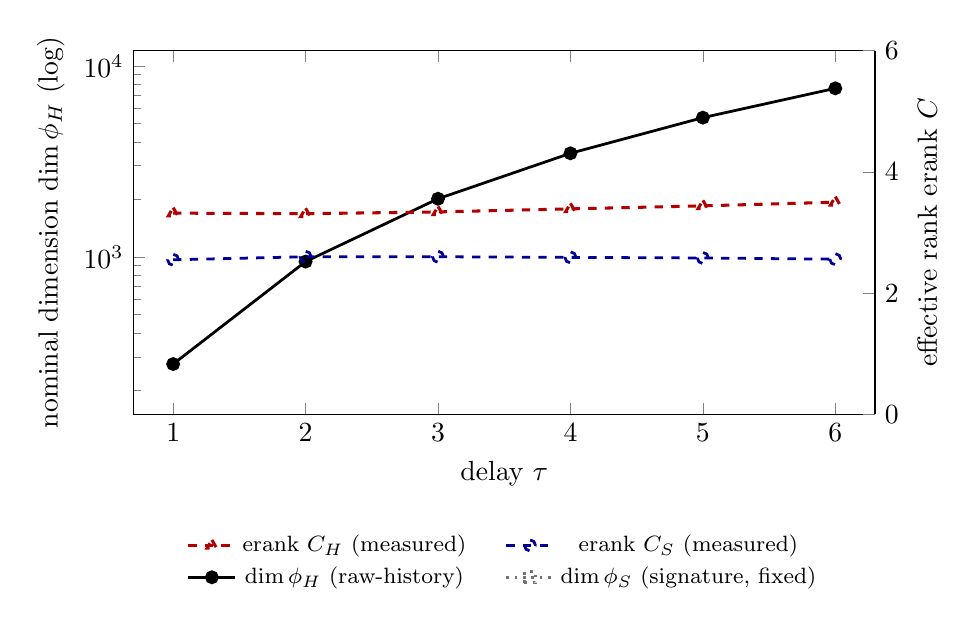
\begin{tikzpicture}
\begin{axis}[
  width=11cm, height=6.2cm,
  xlabel={delay $\tau$}, xmin=0.7, xmax=6.3,
  axis y line*=left, ymode=log, ylabel={nominal dimension $\dim\phi_H$ (log)},
  ymin=150, ymax=12000,
]
\addplot[solid, color=black, mark=*, line width=1.0pt] coordinates {
 (1,275) (2,945) (3,2015) (4,3485) (5,5355) (6,7625)};
\addplot[dotted, color=black!55, mark=square, line width=1.0pt] coordinates {
 (1,30) (2,30) (3,30) (4,30) (5,30) (6,30)};
\end{axis}
\begin{axis}[
  width=11cm, height=6.2cm,
  xmin=0.7, xmax=6.3, axis y line*=right, axis x line=none,
  ylabel={effective rank $\effrank\,C$}, ymin=0, ymax=6,
  legend style={at={(0.5,-0.30)},anchor=north,font=\footnotesize,draw=none,
                legend columns=2,/tikz/every even column/.append style={column sep=12pt}},
]
\addplot[dashed, color=red!70!black, mark=triangle, line width=1.1pt] coordinates {
 (1,3.32) (2,3.31) (3,3.34) (4,3.39) (5,3.44) (6,3.50)};
\addlegendentry{$\effrank\,C_H$ (measured)}
\addplot[dashed, color=blue!60!black, mark=o, line width=1.0pt] coordinates {
 (1,2.55) (2,2.60) (3,2.60) (4,2.59) (5,2.58) (6,2.56)};
\addlegendentry{$\effrank\,C_S$ (measured)}
\addlegendimage{solid, color=black, mark=*, line width=1.0pt}\addlegendentry{$\dim\phi_H$ (raw-history)}
\addlegendimage{dotted, color=black!55, mark=square, line width=1.0pt}\addlegendentry{$\dim\phi_S$ (signature, fixed)}
\end{axis}
\end{tikzpicture}
\caption{The mechanism in one figure. The raw-history nominal dimension (solid, left log axis)
grows by $28\times$ over $\tau\in\{1,\dots,6\}$; the on-manifold effective rank (dashed, right
linear axis) rises only from $3.3$ to $3.5$. The controlled trajectory occupies a ${\sim}3$-dimensional
set regardless of how many feature coordinates encode it, in accordance with the Veronese bound
of Proposition~\ref{prop:veronese}. Solid = nominal dimension; dashed = measured effective rank;
dotted = the signature's fixed dimension.}\label{fig:effrank}
\end{figure}

\begin{observation}[The off-sheet budget scales with the feature dimension: the sample-efficiency law]\label{obs:budget}
Gradient identifiability requires $\ker G_n=\{0\}$ (Proposition~\ref{prop:kerG}). The on-sheet
Gram has rank equal to the effective rank $r^\ast=\effrank C\approx 3.4$
(Finding~\ref{find:effrank}, the Veronese bound of Proposition~\ref{prop:veronese}), so its
co-rank is $\dim\phi-r^\ast$. Off-sheet windows supply the missing rows, each raising
$\rank G_n$ by at most one; reaching full rank therefore needs
\[
  n_{\mathrm{off}}\ \gtrsim\ \dim\phi-r^\ast\ =\ \dim\phi\,\bigl(1+o(1)\bigr)
  \qquad (\dim\phi\to\infty).
\]
The off-sheet perturbations are of small amplitude, hence non-generic, so each contributes less
than a full unit of rank and the measured threshold is $n_{\mathrm{off}}\gtrsim c\,\dim\phi$ with
$c\approx 2$ (the off/dim${}\approx 2$ transition of Table~\ref{tab:controls}), not $c=1$.
Since the signature dimension is fixed while the degree-two history dimension grows as
$\dim\phi_H=O(\tau^{2})$ (window length $L=O(\tau)$, $\dim\phi_H=O((Ln)^{2})$),
\[
  n_{\mathrm{off}}^{\,\mathrm{sig}}=O(1),\qquad
  n_{\mathrm{off}}^{\,\mathrm{raw}}=O(\tau^{2})\qquad (\tau\to\infty).
\]
This is the quantitative content of the sample-efficiency advantage (Observation~\ref{obs:h2}):
the signature is not more expressive; the off-sheet data it requires for identifiability is
independent of the delay, whereas the history window's grows quadratically. The statement is
falsifiable --- it predicts, for any $\tau$, the off-sheet count at which the history fit
recovers --- and is corroborated by the off/dim${}\gtrsim 2$ transitions measured on both the
Hopfield and the Mackey--Glass examples.
\end{observation}

\begin{finding}[On-sheet data identifies only the low-dimensional critic; off-sheet data is a shared precondition]\label{find:onsheet-shared}
The effective rank of the on-sheet (controlled-trajectory) data is $\approx3.4$
(Finding~\ref{find:effrank}), so any representation whose feature dimension exceeds $\approx3.4$ is
under-determined by on-sheet data alone: the value fits ($R^{2}\to1$) while the gradient transverse
to the trajectory is unconstrained (Proposition~\ref{prop:kerG}). This is measured directly on the
Hopfield example with on-sheet data only, over five seeds (Table~\ref{tab:onsheet}), extending the
canonical on-sheet-only comparison of Finding~\ref{find:onsheet} to the primary nonlinear-delayed
example and tying it to the rank. Only the dimension-$5$ markovian critic --- whose dimension is
close to the attractor rank --- is identifiable and stabilises the plant ($I=0.13$ at $\tau=0.5$
and $0.64$ at $\tau=2$, against the oracle $0.09$ and $0.21$); both high-dimensional
representations diverge ($I\sim3$--$4\times10^{2}$, all five seeds), exceeding even the no-control
cost ($I^{0}=9.85$ and $33.5$). The decisive case is $\tau=0.5$, where raw-history is
\emph{over-sampled in count} ($n/\dim=40$) yet still diverges: the obstruction is the
rank-$\approx3.4$ degeneracy of the data, not the sample size. Off-sheet (off-manifold) data is
therefore a precondition \emph{shared by both} high-dimensional representations, and this shared
precondition --- not any property of the signature --- is the reason on-sheet-only fits fail.
\end{finding}

\begin{table}[ht]\centering\small
\caption{Hopfield on-sheet-only (no off-sheet data): closed-loop $I$, mean${}\pm{}$half the $95\%$
confidence interval over five seeds (\texttt{data/h1h2\_hopfield\_onsheet\_5seed}). Only the
dimension-$5$ markovian critic (dimension near the on-sheet effective rank $\approx3.4$) is
identifiable; both high-dimensional representations diverge --- the signature marginally worse than
raw-history --- above even the no-control cost $I^{0}$. At $\tau=0.5$ raw-history has $n/\dim=40$,
so the divergence is the rank degeneracy, not a sample shortage.}\label{tab:onsheet}
\setlength{\tabcolsep}{6pt}
\begin{tabular}{cl ccc}
\toprule
$\tau$ ($I^{0}\!\to\! I^{\ast}$) & rep & $\dim\phi$ & $n/\dim$ & $I$ (mean $\pm$ ci)\\
\midrule
\multirow{3}{*}{$0.5$ ($9.85\!\to\!0.09$)}
 & markovian   & 5  & 726  & $\mathbf{0.131\pm0.012}$\\
 & raw-history & 90 & 40.3 & $318\pm8$\\
 & signature   & 30 & 121  & $393\pm10$\\
\midrule
\multirow{3}{*}{$2.0$ ($33.5\!\to\!0.21$)}
 & markovian   & 5   & 726 & $\mathbf{0.642\pm0.18}$\\
 & raw-history & 945 & 3.8 & $371\pm27$\\
 & signature   & 30  & 121 & $415\pm11$\\
\bottomrule
\end{tabular}
\end{table}

\begin{observation}[The shared precondition sets up the efficiency distinction, not an expressivity gap]\label{obs:precond}
Finding~\ref{find:onsheet-shared} is the precondition common to both high-dimensional maps; they
differ only in \emph{how much} off-sheet data restores them. Given off-sheet data, the scaling
sweeps (Table~\ref{tab:controls}, Table~\ref{tab:generality}) show the signature needs less: its
fixed dimension ($\sim30$) is over-determined already at the smallest off-sheet budget, whereas
raw-history's $O(\tau^{2})$ dimension requires off/dim${}\gtrsim2$ against its own growing count.
Once that adequate, balanced off-sheet data is supplied, raw-history converges and matches or beats
the signature on every example (Findings~\ref{find:controls} and~\ref{find:mg}). The signature's
advantage is therefore sample efficiency and conditioning, not expressivity: both high-dimensional
representations require off-sheet data; the signature simply requires less of it.
\end{observation}

\subsection{Synthesis}

\begin{observation}[The signature trades a delay blow-up for a dimension blow-up]\label{obs:synthesis}
The two representations encode the \emph{same} low-effective-rank object
(Proposition~\ref{prop:veronese}, Finding~\ref{find:effrank}) with differently growing numbers
of coordinates. The raw-history dimension grows with the \emph{delay} as $O((L n)^{2})=O(\tau^2)$
(Table~\ref{tab:catalogue}, Hopfield $90\to7625$); the signature dimension grows with the
\emph{state dimension} as $O(d^{L})$ (platoon $12\to462$). Neither growth adds representational
power; each is an over-parameterisation that the off-sheet data must condition. Hence the
measured pattern: the signature's fixed delay-dimension helps on long-delay, low-state-dimension
examples \emph{when data are scarce} (its sample-efficiency advantage), and its channel growth hurts
on the high-state-dimension platoon (where $\gamma_S=0.32$ and $I_S=0.227$ exceed even the
markovian critic). Given off-sheet data balanced to the representation's dimension
(off/dim${}\gtrsim2$), the degree-two history window matches or beats the signature on every example
measured. The signature's genuine advantage is sample efficiency, not representational power.
\end{observation}

\section{Conclusion}\label{sec:conclusion}

The history of the state is a genuine and robust ingredient of optimal control for delayed
plants: $H_1$ holds, measured and seed-stable, on every example where the delay couples the
dynamics, and fails exactly on the Markovian negative control and on the near-Markovian Dadebo
reactor (demoted on the measured history-kernel ratio). Where the comprehensive \emph{learned}
benchmark reports $H_1$ failing on an ill-conditioned example, the controlled plain-least-squares
protocol shows the cause to be under-convergence of the high-dimensional history representation,
not a representational deficit: the learned and controlled instruments agree once conditioning is
accounted for. The path-signature
\emph{structure}, by contrast, confers no representational advantage over a plain degree-two
polynomial of the history window: every apparent advantage is an artefact of the history map being
under-sampled at long delay, and is removed by more data, by conditioning, or by off-sheet
rebalancing. The mechanism is the effective-rank phenomenon --- proven as a Veronese bound,
measured as a flat effective rank against a $28\times$ dimension growth --- which makes both
representations over-parameterisations of a ${\sim}3$-dimensional controlled-trajectory object.
The signature's one real benefit is a fixed feature dimension, i.e.\ sample efficiency at long
delay and low state dimension; that benefit reverses at high state dimension, where the
signature's own channel growth makes it the ill-conditioned choice. For deployment, the
operative levers are off-manifold (off-sheet) data design and conditioning, not a richer feature
algebra.

\appendix

\section{Visualisation: controlled trajectories and control signals}\label{app:viz}

\emph{Each figure overlays, from the example's deployment initial condition, the closed-loop state
$x_0(t)$ (top) and control $u_0(t)$ (bottom) of the three critics against the analytic oracle
reference and the no-control response. The critics are fitted on exactly the benchmark data
(same seed, same protocol); the local closed-loop cost reproduces the cluster
\texttt{summary.json} value (e.g.\ linear\_dde markovian/raw/signature $0.366/0.152/0.201$,
matching the canonical seed-0 fit to four decimals), so these are faithful regenerations.
Convention: \emph{solid} = learned critics, \emph{dashed} = analytic oracle, \emph{dotted} =
no control.}

\begin{figure}[ht]\centering
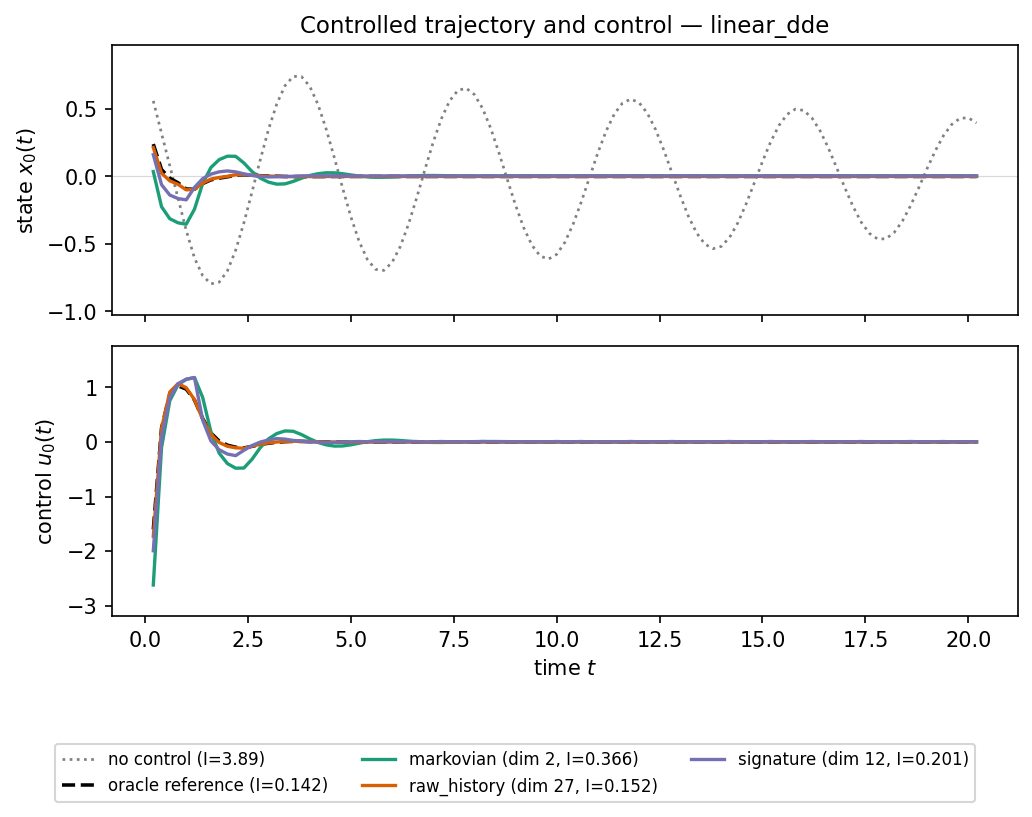
\includegraphics[width=0.82\textwidth]{figures/traj_linear_dde.png}
\caption{\texttt{linear\_dde}. $H_1$ visible: the markovian critic (green) overshoots and settles
slowly; the history window (orange) tracks the oracle and attains the lowest cost; the signature
(purple) is marginally worse ($H_2$ fails). The no-control response (dotted) sustains an
oscillation.}\label{fig:traj-linear}
\end{figure}

\begin{figure}[ht]\centering
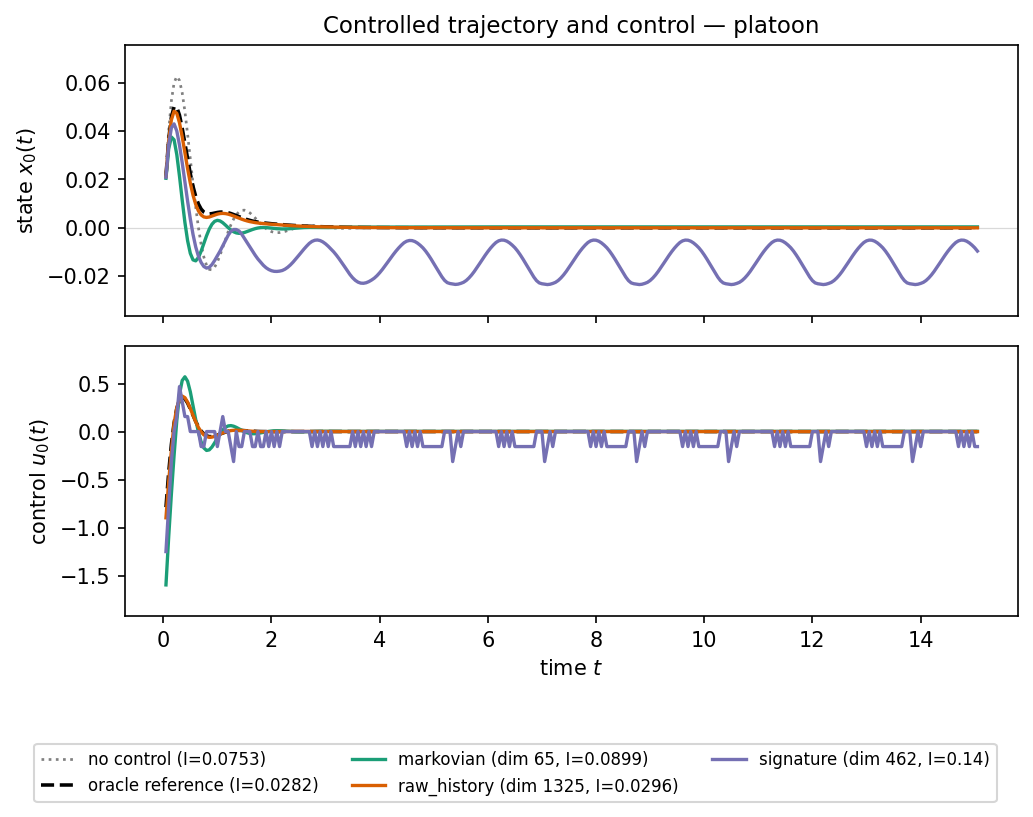
\includegraphics[width=0.82\textwidth]{figures/traj_platoon.png}
\caption{\texttt{platoon}. The decisive $H_2$ failure: the history window (orange, dimension
$1325$) tracks the oracle and settles; the signature (purple, dimension $462$) \emph{sustains an
undamped oscillation} it never regulates, its control signal (bottom) saturating --- the
ill-conditioned gradient ($\gamma_S=0.32$, condition number ${\sim}10^{14}$) producing a wrong
feedback despite a near-perfect value fit ($R^2=0.999$).}\label{fig:traj-platoon}
\end{figure}

\begin{figure}[ht]\centering
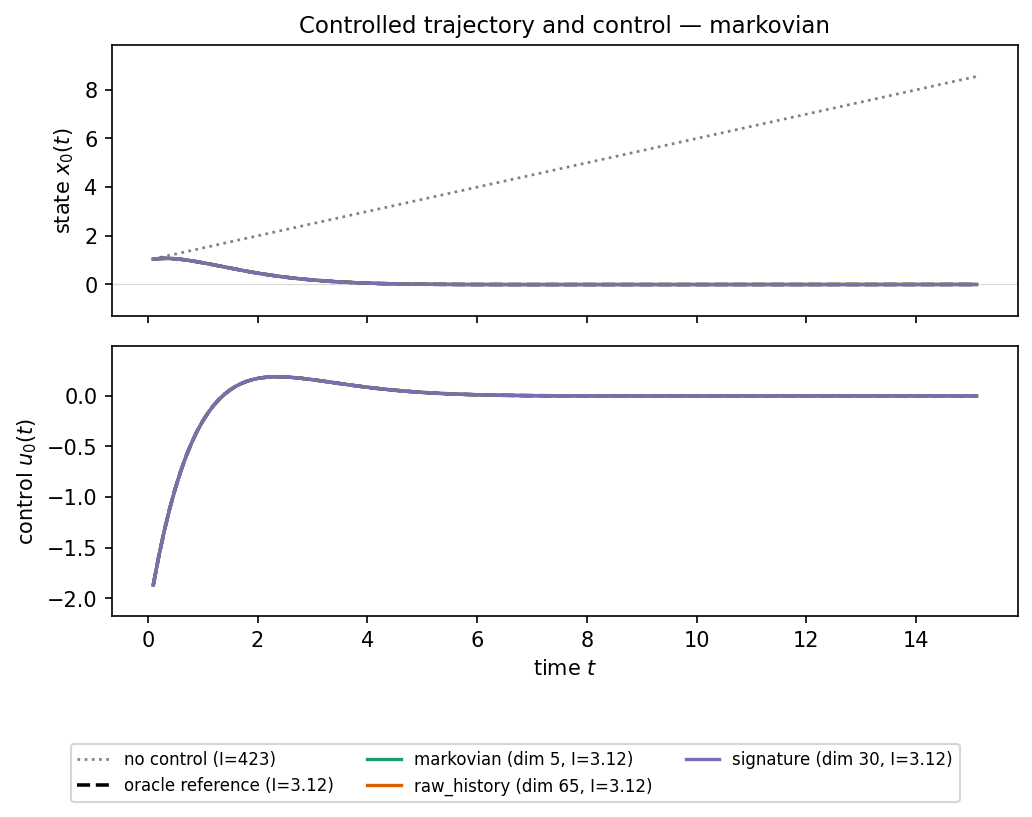
\includegraphics[width=0.49\textwidth]{figures/traj_markovian.png}\hfill
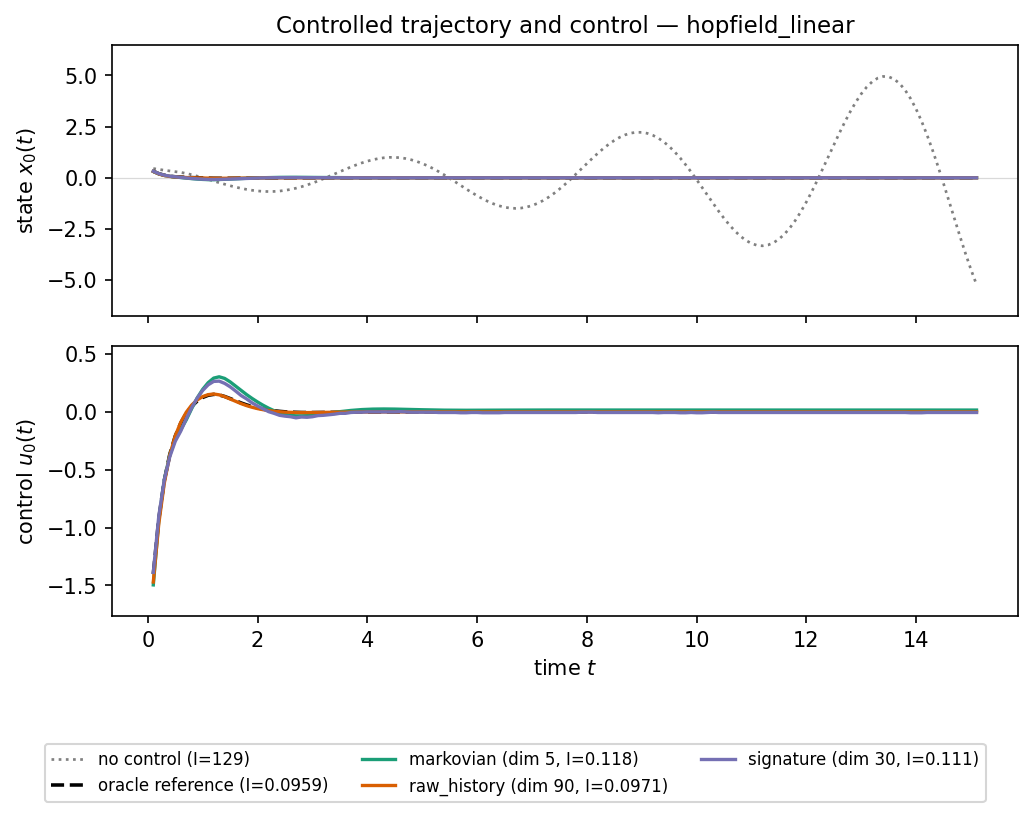
\includegraphics[width=0.49\textwidth]{figures/traj_hopfield_linear.png}
\caption{Left, \texttt{markovian} negative control: the three critics coincide (history
irrelevant). Right, \texttt{hopfield\_linear}: $H_1$ holds (history window below markovian),
$H_2$ fails (signature above history window) --- the provable-negative linear-in-delay
arm.}\label{fig:traj-extra}
\end{figure}

\begin{figure}[ht]\centering
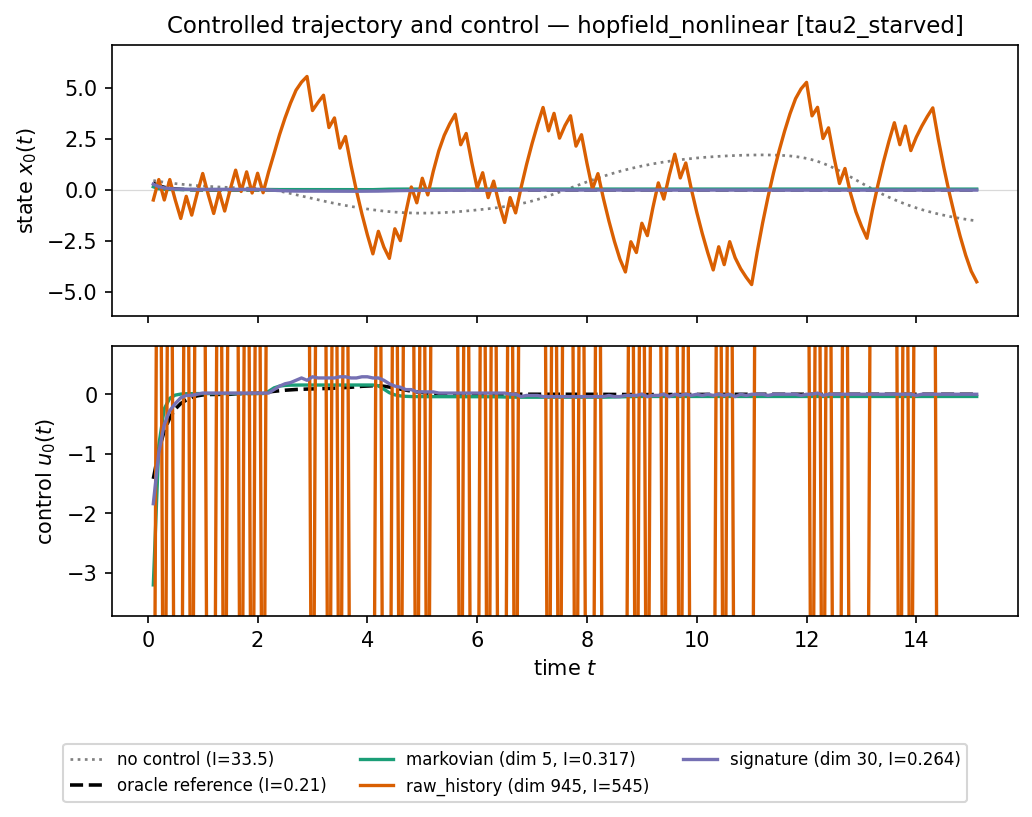
\includegraphics[width=0.49\textwidth]{figures/traj_hopfield_tau2_starved.png}\hfill
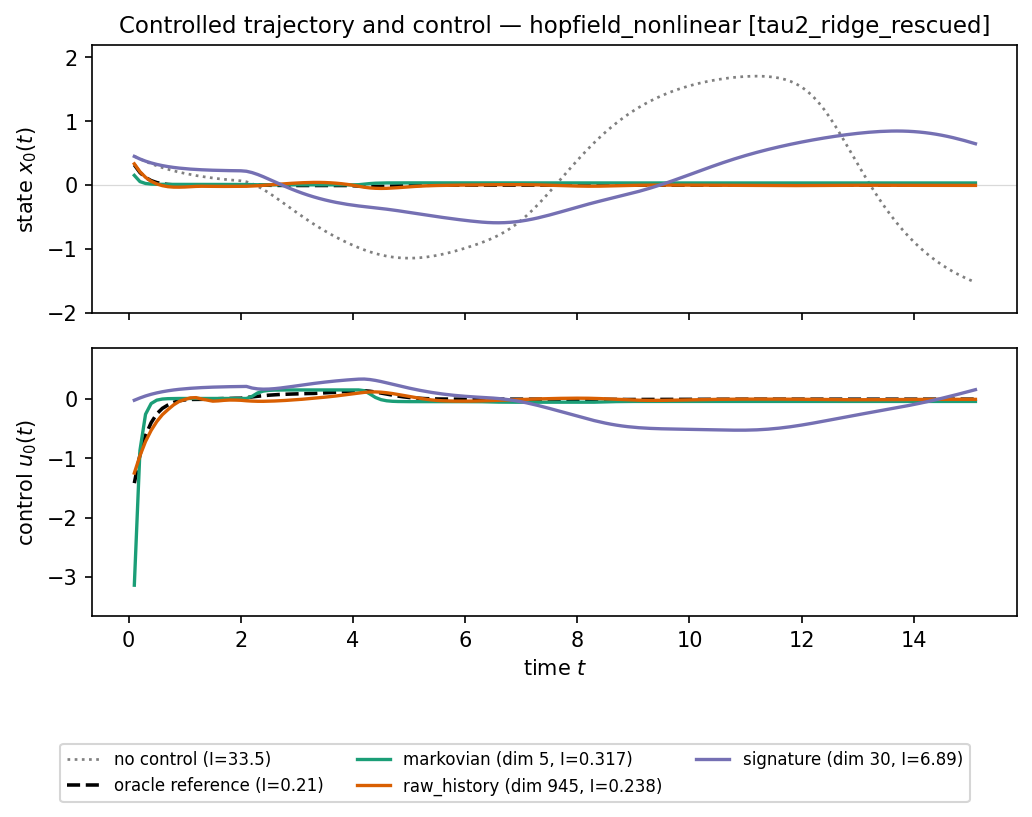
\includegraphics[width=0.49\textwidth]{figures/traj_hopfield_tau2_rescued.png}
\caption{\texttt{hopfield\_nonlinear} at $\tau=2$: the $H_2$ illusion and its cure. Left, the
under-sampled fit ($n/\dim\phi_H=4.4$): the history window (orange, dimension $945$) diverges into a
saturating bang-bang control ($I=545$) while the signature (purple) and oracle (dashed) track,
so the signature appears preferable. Right, the same data with Tikhonov conditioning
($\lambda=10^{-2}$): the history window is restored to $I=0.238$ and tracks the oracle, while the
identical ridge over-damps the signature ($I=6.89$). The cure is conditioning, not capacity
(Finding~\ref{find:controls}).}\label{fig:traj-bvp}
\end{figure}

\begin{figure}[ht]\centering
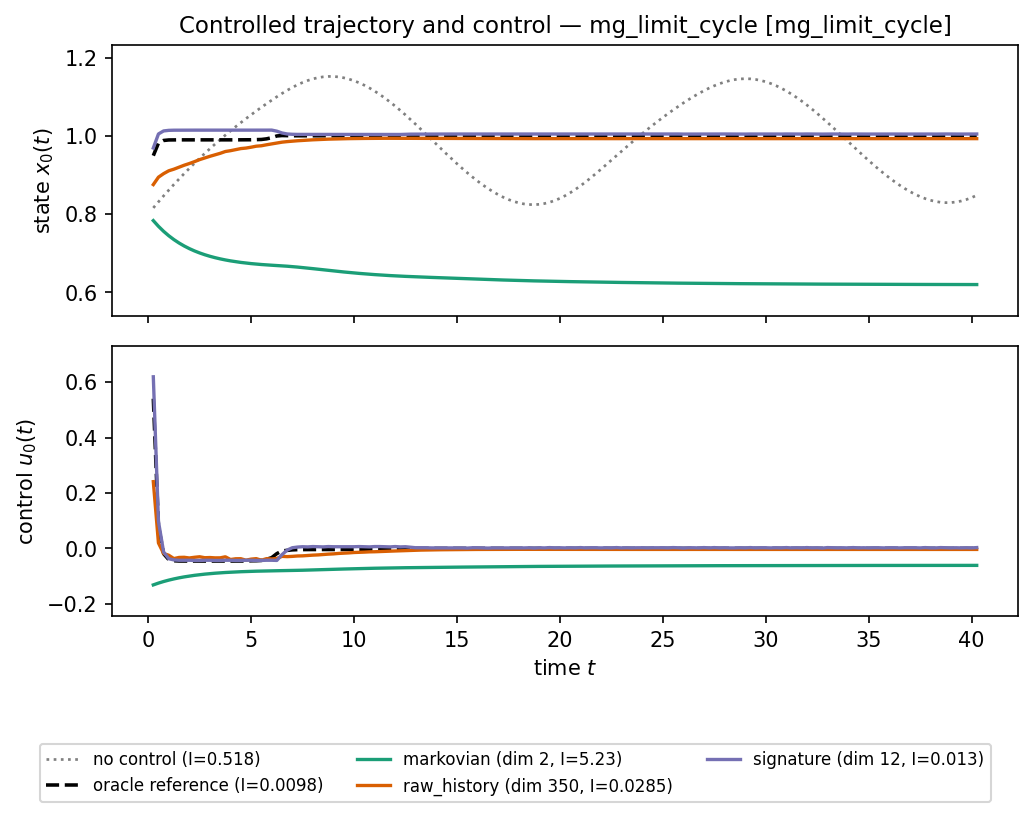
\includegraphics[width=0.78\textwidth]{figures/traj_mg_limit_cycle.png}
\caption{\texttt{mg\_limit\_cycle} (canonical off-sheet budget, $N_{\mathrm{off}}=500$). A clean
$H_1$ picture: the markovian critic (green) cannot represent the value
($R^{2}=0.14$) and drives the state to a \emph{wrong} equilibrium near $x_0=0.62$ (cost
$I=5.23$), while the history window (orange) and signature (purple) both regulate to
$x^{\ast}=1$. At this off-sheet budget the signature leads ($I=0.013$ versus the history
window's $0.029$); Finding~\ref{find:mg} shows that scaling the off-sheet data to off/dim${}=4$
reverses the ordering.}\label{fig:traj-mg}
\end{figure}

\section{Learning-half confirmation (LSPI)}\label{app:rl}

\emph{The oracle half is the primary evidence; the damped-LSPI learning half confirms it under a
temporal-difference estimator rather than a supervised one. These runs are single-seed
(the full learning-half matrix was cancelled on a storage quota), so they are confirmatory, not
falsifiable. The reg${}=10^{-4}$ conditioning fix of the parallel code is in effect.}

\begin{table}[ht]\centering\small
\caption{Learning half (damped LSPI), closed-loop $I$, single seed
(\texttt{h1h2\_rl\_lspi}). $H_1$ holds on the delay examples and fails on the Markovian negative
control, mirroring Table~\ref{tab:h1}.}\label{tab:rl}
\setlength{\tabcolsep}{6pt}
\begin{tabular}{lccc c}
\toprule
example & $I_M$ & $I_H$ & $I_S$ & $H_1$\\
\midrule
markovian (neg.\ control) & 3.782 & 3.687 & 3.849 & \failsv\\
linear\_dde               & 0.423 & 0.181 & 0.128 & \holds\\
hopfield\_linear          & 0.134 & 0.108 & 0.111 & \holds\\
hopfield\_duffing         & 0.147 & 0.118 & 0.115 & \holds\\
\bottomrule
\end{tabular}
\end{table}

\begin{observation}[The learning half agrees on $H_1$; $H_2$ is inconclusive single-seed]\label{obs:rl}
Table~\ref{tab:rl} reproduces the $H_1$ verdict: history lowers $I$ on every delay example and not
on the Markovian control. On $H_2$ the single-seed learning runs are mixed (signature marginally
below history on linear\_dde and hopfield\_duffing, marginally above on hopfield\_linear) and at
the $3\%$ margin are within run-to-run variation; no falsifiable $H_2$ claim is made from the
learning half. The oracle half (Section~\ref{sec:h2}), with five seeds and the controls, is the
operative evidence.
\end{observation}

\section{Robustness of the comprehensive benchmark}\label{app:robust}

\emph{Three control studies on the high-gap oscillator support the readings of
Section~\ref{sec:mainunified}: an oracle ladder isolating the actor/critic contributions to the
residual cost, a training-trick ablation, and a budget sweep. All use the learned pipeline; costs
are the best-iterate evaluation cost $J$ (not the normalised $\rho$), so they are compared only
within each study.}

\begin{table}[ht]\centering\small
\caption{Left: oracle ladder (\texttt{oracle\_ladder\_high\_gap}, 3 seeds) --- evaluation cost
with the actor and/or critic replaced by the oracle. Right: budget sweep
(\texttt{budget\_sweep\_high\_gap}, 2 seeds) --- evaluation cost versus training episodes.}
\label{tab:robust}
\setlength{\tabcolsep}{6pt}
\begin{minipage}[t]{0.52\textwidth}\centering
\begin{tabular}{lc}
\toprule
configuration & $J$ (best iterate)\\
\midrule
full learned (actor + critic)  & $2.82\pm0.08$\\
oracle critic, learned actor   & $2.56\pm0.03$\\
oracle actor, learned critic   & $1.83\pm0.00$\\
\bottomrule
\end{tabular}\\[2pt]
{\footnotesize Replacing the actor cuts the cost most ($2.82\to1.83$), the critic less
($2.82\to2.56$): the residual is dominated by policy (gradient) extraction, consistent with the
value/gradient gap of Proposition~\ref{prop:kerG}.}
\end{minipage}\hfill
\begin{minipage}[t]{0.44\textwidth}\centering
\begin{tabular}{lcc}
\toprule
budget & markovian$_2$ & raw-history$_2$\\
\midrule
800   & 3.22 & 2.60\\
2400  & 3.22 & 2.46\\
7200  & 3.22 & 2.32\\
\bottomrule
\end{tabular}\\[2pt]
{\footnotesize Raw-history keeps converging with budget; markovian is flat
(representation-limited). Evidence that the learned $H_1$ failure on this example is
under-convergence (Finding~\ref{find:underconv}).}
\end{minipage}
\end{table}

\begin{observation}[The convergence is robust to the training tricks]\label{obs:trick}
A five-way ablation of the stabilisers (\texttt{trick\_ablation\_convergence}, 3 seeds) leaves
both the convergence speed and the final cost within a narrow band: episodes to the
$\rho=0.1$ threshold are $160$--$190$, and the final $\rho$ is $0.025$ (minimal, no-target-net)
to $0.036$ (baseline, no-divergence-threshold, white-noise). Removing the target network or the
divergence threshold does not break convergence; injecting white observation noise does not
change the final cost beyond the seed band. The benchmark's verdicts are not artefacts of a
particular training stabiliser.
\end{observation}

\section{Reproduction}\label{app:repro}

\emph{Every number and figure traces to a saved run. Scripts are in
\texttt{run/study/}; oracle-half run directories are under
\texttt{data/h1h2\_evaluation/} (cluster \texttt{\$WORK}) and the $\tau$/control sweeps under the
cluster \texttt{\$SCRATCH} (\texttt{/lustre/fsn1/projects/rech/oym/ucd32aq}); they are
consolidated locally under \texttt{data/h1h2\_report\_runs/}.}

\paragraph{Scripts.}
\begin{itemize}\setlength{\itemsep}{1pt}
\item \texttt{h1h2\_evaluation.py} --- oracle-half harness (examples, oracle, data protocol, plain
least squares, three metrics). Tables~\ref{tab:h1},~\ref{tab:tausweep},~\ref{tab:controls},~\ref{tab:generality}.
\item \texttt{h1h2\_rl\_lspi.py} --- learning-half (damped LSPI). Table~\ref{tab:rl}.
\item \texttt{h1h2\_effective\_rank\_vs\_delay.py} --- on-manifold effective rank versus delay.
Table~\ref{tab:effrank}, Figure~\ref{fig:effrank}.
\item \texttt{h1h2\_visualise\_controlled\_trajectories.py} --- closed-loop trajectory/control
figures (Appendix~\ref{app:viz}); regenerates from saved \texttt{.npz}.
\item Solvers: \texttt{src/solvers/continuous\_oracle.py} (delayed-LQR),
\texttt{\{mackey\_glass,delayed\_hopfield\}\_pontryagin.py} (nonlinear oracle).
\end{itemize}

\paragraph{Run directories.} All consolidated read-only under \texttt{data/h1h2\_report\_runs/}
(index in \texttt{INDEX.md}); pulled from Jean Zay \texttt{\$WORK} (learned/oracle) and
\texttt{\$SCRATCH} (sweeps).
\begin{itemize}\setlength{\itemsep}{1pt}
\item Comprehensive learned benchmark (Section~\ref{sec:mainunified},
Table~\ref{tab:mainunified}): \texttt{main\_unified/} --- per-example sub-studies
(\texttt{*\_study/summary.yaml}) sweeping capacity $\times$ 5 seeds. Robustness
(Appendix~\ref{app:robust}): \texttt{main\_unified/\{oracle\_ladder\_high\_gap,
trick\_ablation\_convergence, budget\_sweep\_high\_gap\_b*\}}.
\item Canonical $H_1/H_2$ (5 examples $\times$ 5 seeds): \texttt{20260616\_161650\_on\_off\_sheet\_array}
(Table~\ref{tab:h1}); on-sheet-only twin \texttt{20260616\_161649\_on\_sheet\_array}
(Finding~\ref{find:onsheet}).
\item Hopfield: \texttt{h1h2\_tau\_sweep\_20260617\_165104} (Table~\ref{tab:tausweep});
\texttt{h1h2\_tau2\_control\_20260617\_171721}, \texttt{h1h2\_tau2\_ridge\_20260617\_180843},
\texttt{h1h2\_tau3\_control\_20260617\_194242}, \texttt{h1h2\_tau3\_offsheet\_20260617\_204438}
(Table~\ref{tab:controls}, Finding~\ref{find:balance}).
\item Duffing: \texttt{h1h2\_duffing\_kappa\_sweep\_20260617\_155613}; Mackey--Glass off-sheet:
\texttt{h1h2\_mg\_offsheet\_20260630\_164840} (Table~\ref{tab:generality}).
\item Effective rank: \texttt{data/h1h2\_effective\_rank\_vs\_delay/} (Table~\ref{tab:effrank}).
Hopfield on-sheet-only (5 seeds): \texttt{data/h1h2\_hopfield\_onsheet\_5seed/}
(Table~\ref{tab:onsheet}), produced by \texttt{h1h2\_evaluation.py -\/-data-mode on\_sheet}.
\end{itemize}

\paragraph{Provenance caveats.} The Hopfield/Mackey--Glass sweeps and the effective-rank
measurement are single-seed (the operative quantity there is the data/conditioning axis, not seed
variance); the canonical $H_1/H_2$ table is five-seed. The Mackey--Glass off-sheet curve is now
complete for both examples (the last mg\_chaotic point, off/dim${}=4$, at $\sim10^{4}$ Pontryagin
solves, finished after the first draft and is included). The trajectory
figures are local regenerations whose well-conditioned costs
match the cluster \texttt{summary.json} to four decimals; the ill-conditioned signature on the
platoon reproduces only to ${\sim}10\%$ (local $0.140$ versus cluster $0.164$), itself a symptom
of the condition number of Figure~\ref{fig:traj-platoon}.

\end{document}
